\subsection{Aplicación para Android CloudNAO}
\label{\detokenize{introduction:welcome-to-cloudnao-android-s-documentation}}
Esta aplicación móvil es el componente dentro de la arquitectura CloudNAO
que permite interactuar con el robot sin necesidad de instalar software en el
robot. Se conecta con el robot usando el SDK para Android de NAOqi, hace peticiones
a la API RESTful de CloudNAO, y además utiliza la autenticación
y la base de datos en tiempo real de Firebase utilizando su SDK para Android.

Es una aplicación moderna que no se limita a ser un simple control remoto, y
añade funcionalidades como la escritura de logs generados por el robot en la nube,
y el potente análisis de imágenes simplemente haciendo peticiones a la API
RESTful de CloudNAO.

En las siguientes secciones se describe con mayor detalle cada elemento de la
aplicación, ya sea para la parte que ve el usuario final como los componentes
internos para que desarrolladores puedan mantenerla o añadir nuevas
funcionalidades.

\subsubsection{Descripción de la aplicación}
\paragraph{Requisitos}
\label{\detokenize{users_docs:requisitos}}
La aplicación fue probada con éxito sobre dispositivos con arquitecturas ARM,
y con una versión menor o igual a Android 5.1.1 (API 22). Los problemas con
nuevas plataformas son que el SDK provisto por Aldebaran, no es compatible con
arquitecturas x86, ni con nuevas versiones de Android. Esta incompatibilidad
se debe a la forma en que se compiló el archivo
\sphinxstyleemphasis{java-naoqi-sdk-2.1.4-android.jar}.


\paragraph{Funcionalidades}
\label{\detokenize{users_docs:fucionalidades}}
La aplicación ofrece algunas características que más que nada sirven para
mostrar casos de uso para algunos recursos dentro de la API RESTful
de CloudNAO, y para utilizar productos de Firebase como la autenticación
o la base de datos en tiempo real.

Cabe señalar que al usar a Firebase como BaaS, la aplicación móvil
comparte información con la aplicación web de CloudNAO. Por ejemplo, los
usuarios que se registren en una u otra, pueden iniciar sesión en cualquiera
sin problemas; similar es el caso de los robots que registren y la información
de cada uno.

En general las siguientes son las funcionalidades ofrecidas por las aplicación.


\subparagraph{Autenticación de usuarios.}
\label{\detokenize{users_docs:autenticacion-de-usuarios}}
Para poder ocupar la aplicación los usuarios deben iniciar sesión con un correo
y contraseña. La aplicación cuenta con la opción de registro, si el usuario
es nuevo.


\begin{figure}[!h]
    \centering
    \subfloat{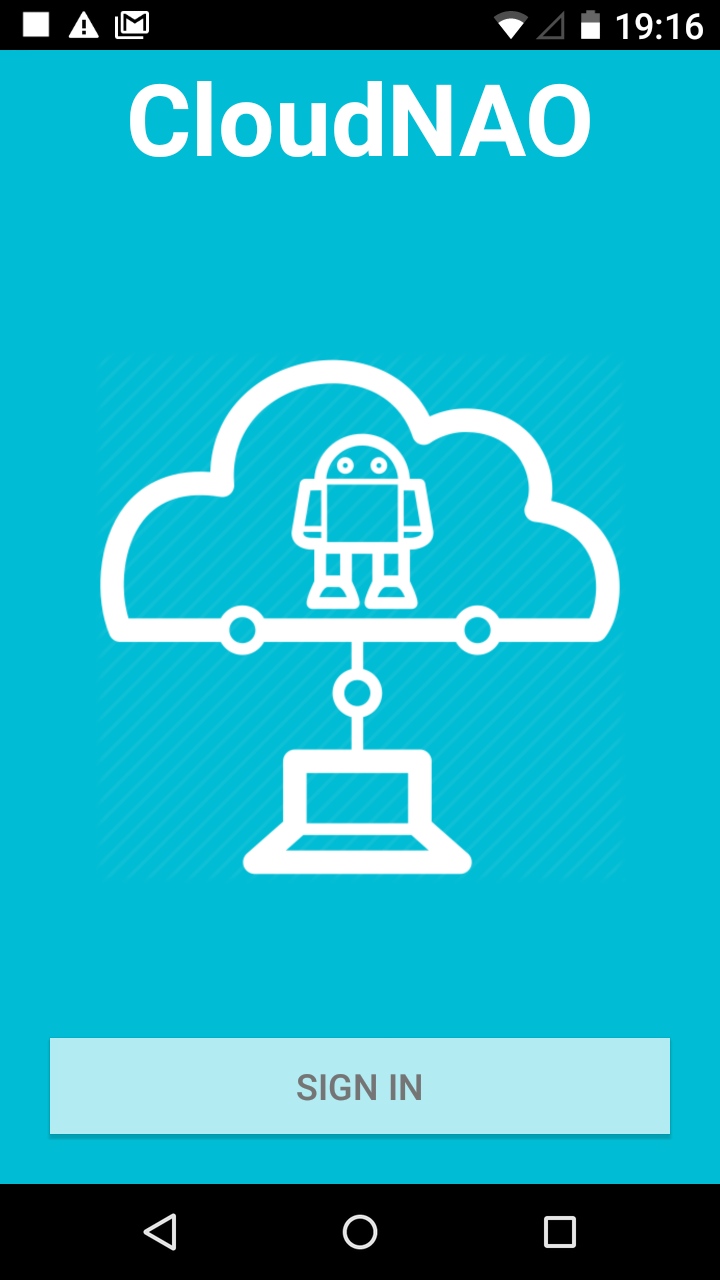
\includegraphics[scale=.1]{signin}}%
    \qquad
    \subfloat{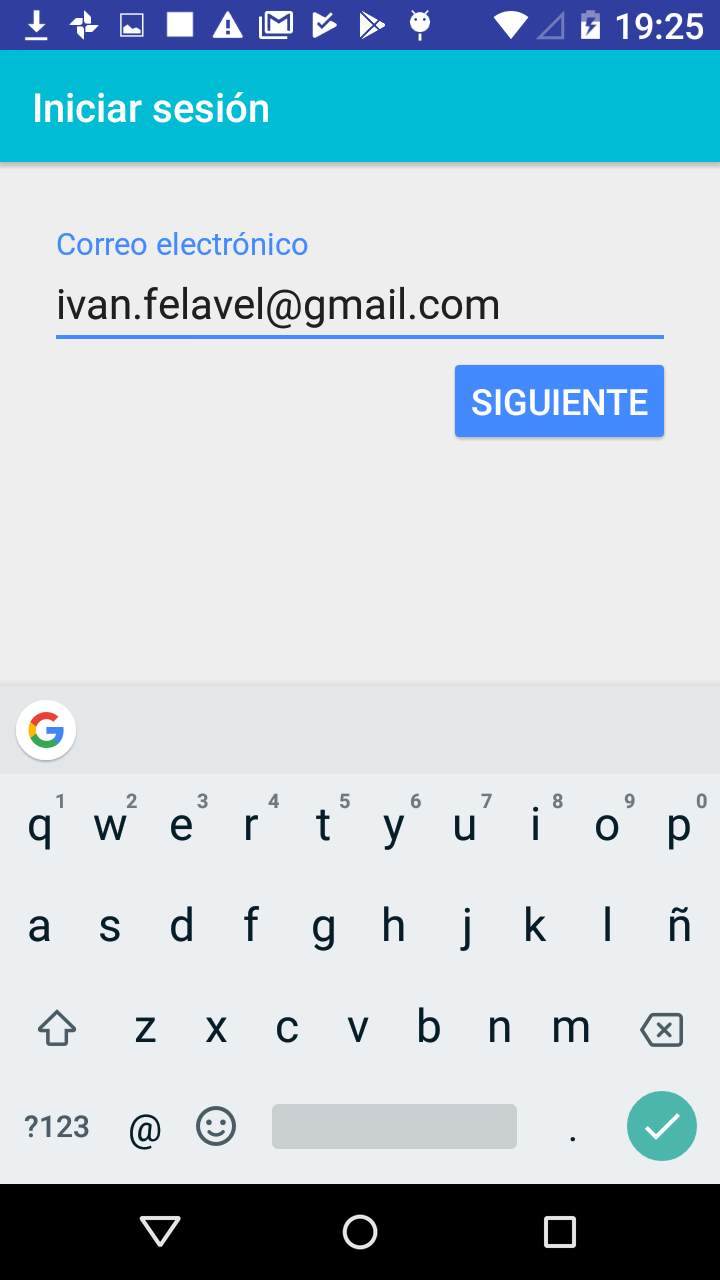
\includegraphics[scale=.1]{signin1}}%
    \qquad
    \subfloat{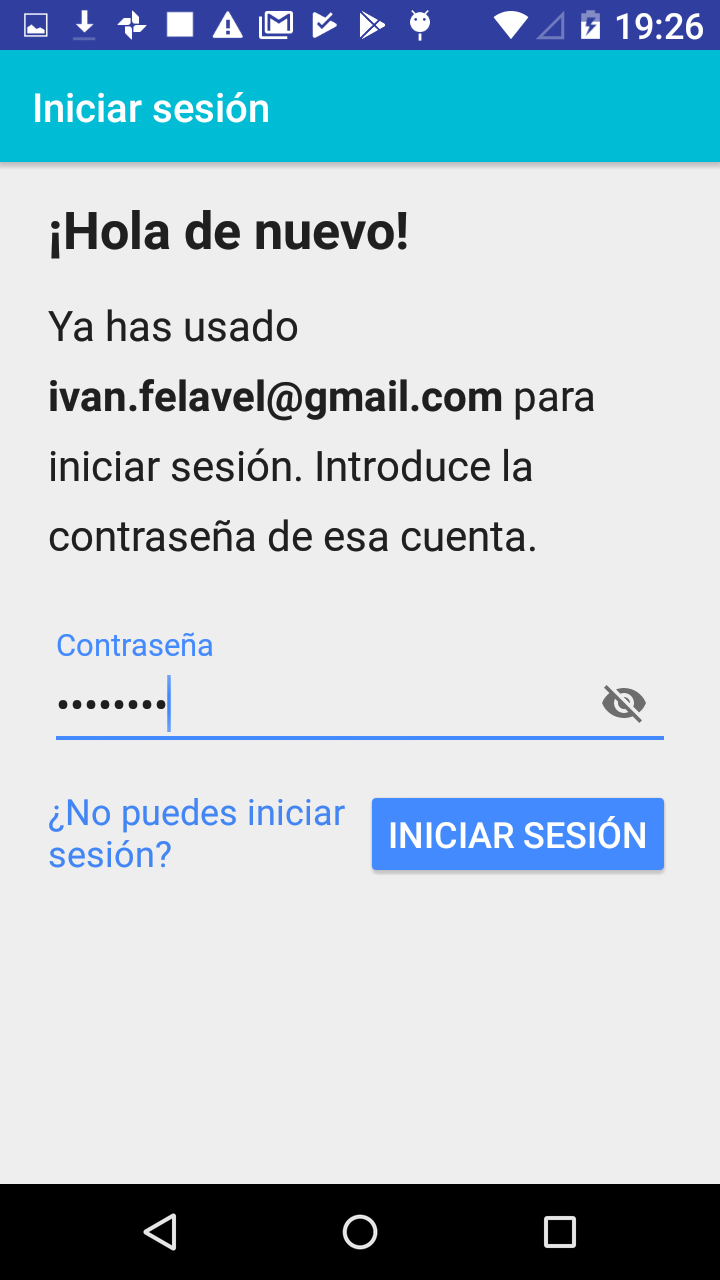
\includegraphics[scale=.1]{signin2}}%
\end{figure}

\subparagraph{Selección y adición de robots a la aplicación.}
\label{\detokenize{users_docs:los-usuarios-pueden-anadir-nuevos-robots}}
Para llevar un control de los robots que tiene un usuario se le permite añadir
los robots que sean necesarios.
Además el usuario cuenta con una lista que le muestra los robots disponibles
que previamente creó.

\begin{figure}[!h]
    \centering
    \subfloat{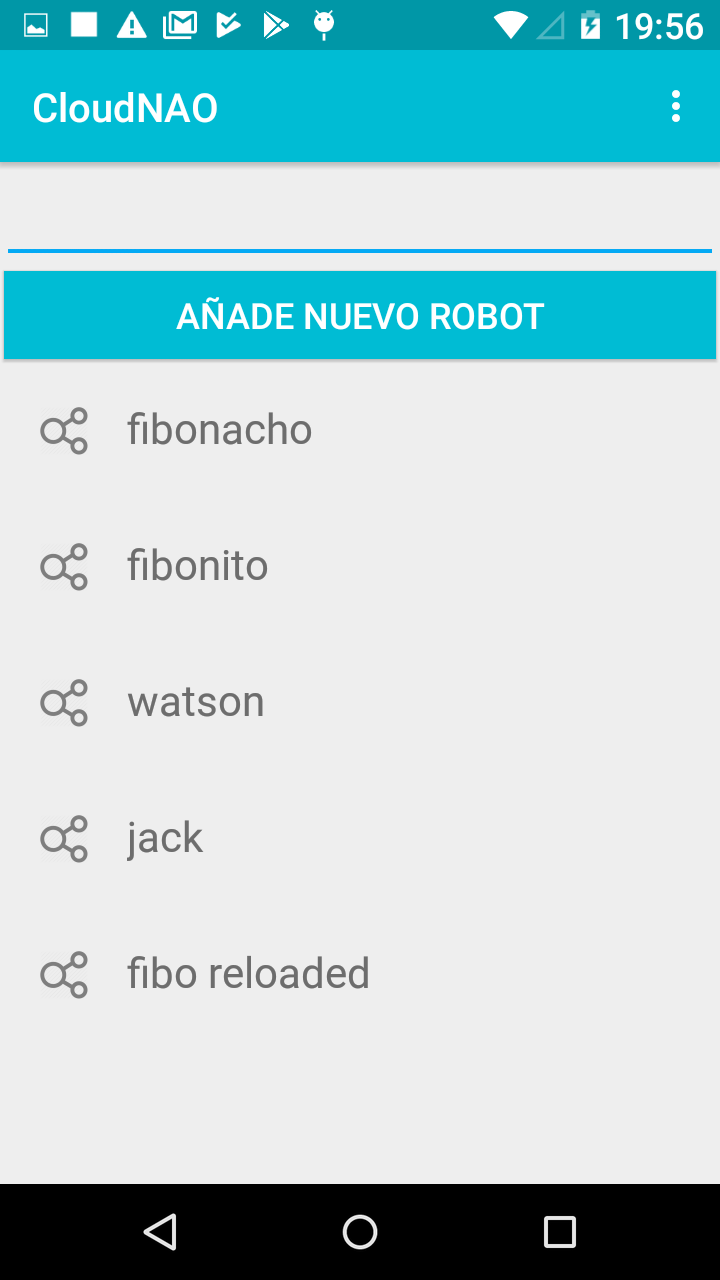
\includegraphics[scale=.1]{add_robot1}}%
    \qquad
    \subfloat{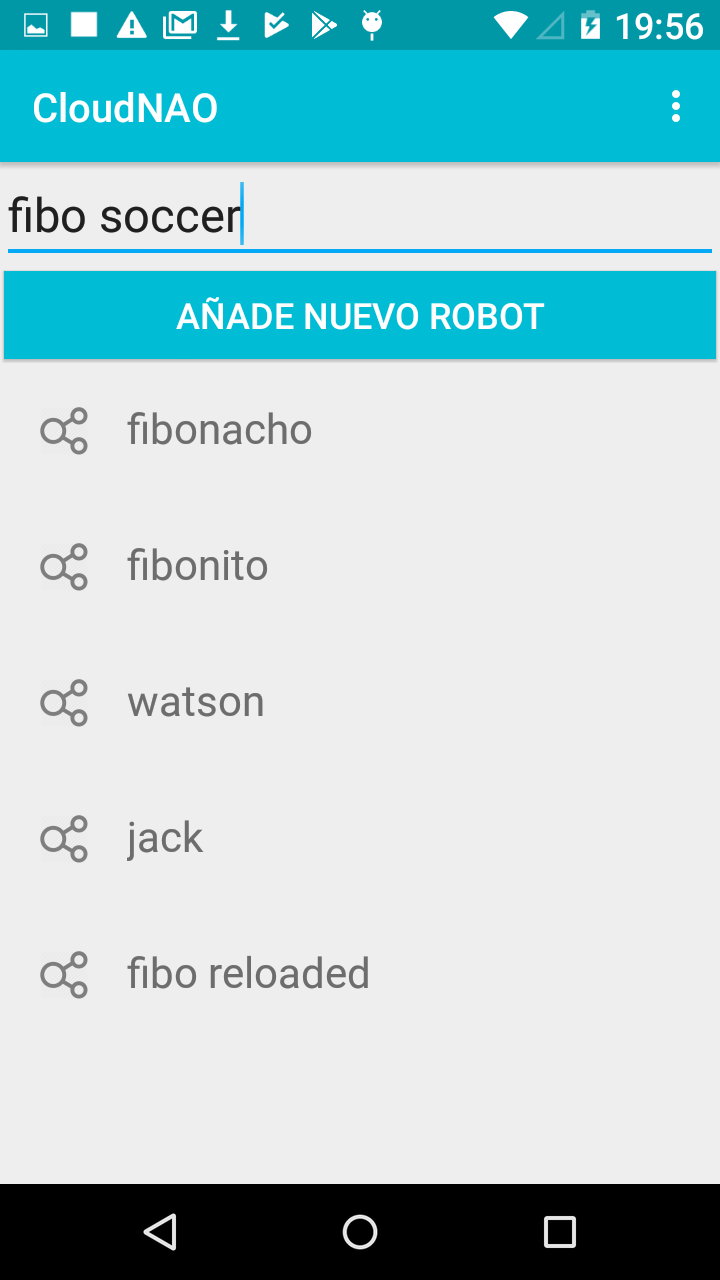
\includegraphics[scale=.1]{add_robot2}}%
    \qquad
    \subfloat{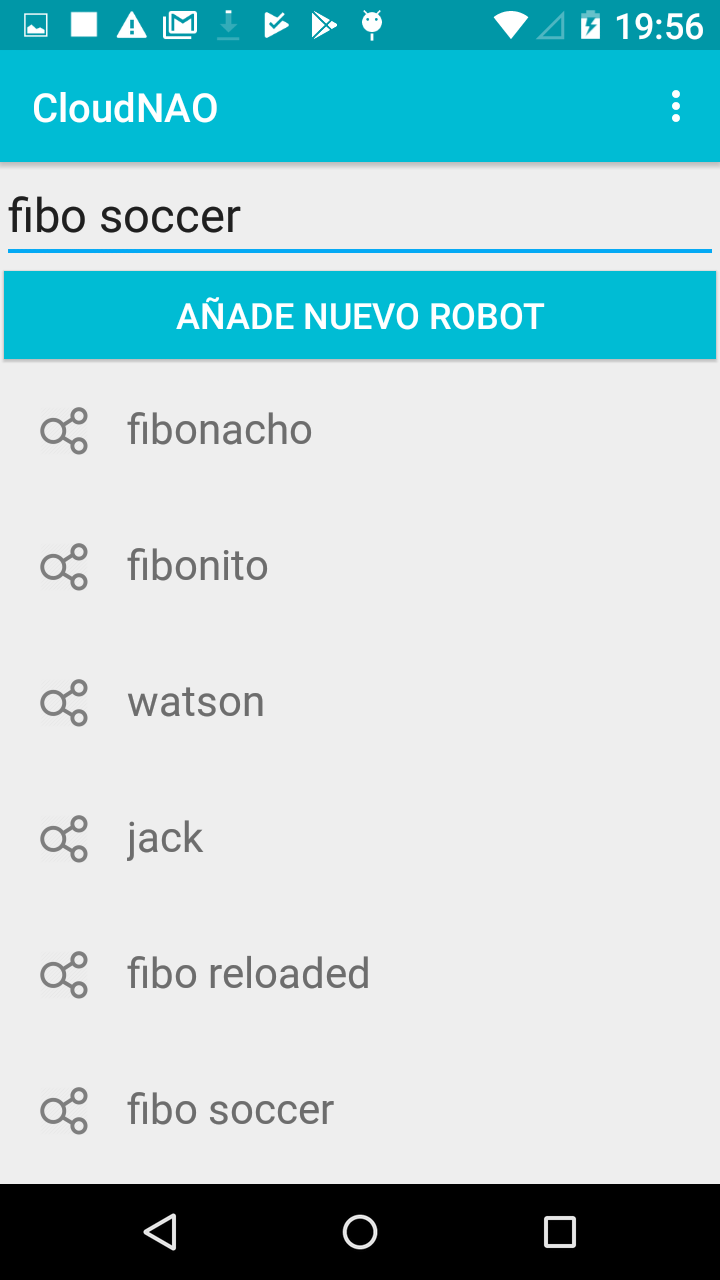
\includegraphics[scale=.1]{add_robot3}}%
    \caption{La aplicación se conecta con Firebase para obtener los
    robot creados y al crear uno se añade a la Firebase Realtime Database.}
    
\end{figure}



\subparagraph{Conexión con un robot seleccionado.}
\label{\detokenize{users_docs:conexion-con-un-robot-seleccionado}}
Al elegir un robot entre los que el usuario posee, simplemente escribe la
dirección IP del robot, y se crea una conexión con éste dentro de la misma
red. Con esto, es posible acceder a todas las características disponibles en la
aplicación.


\begin{figure}[!h]
    \centering
    \subfloat{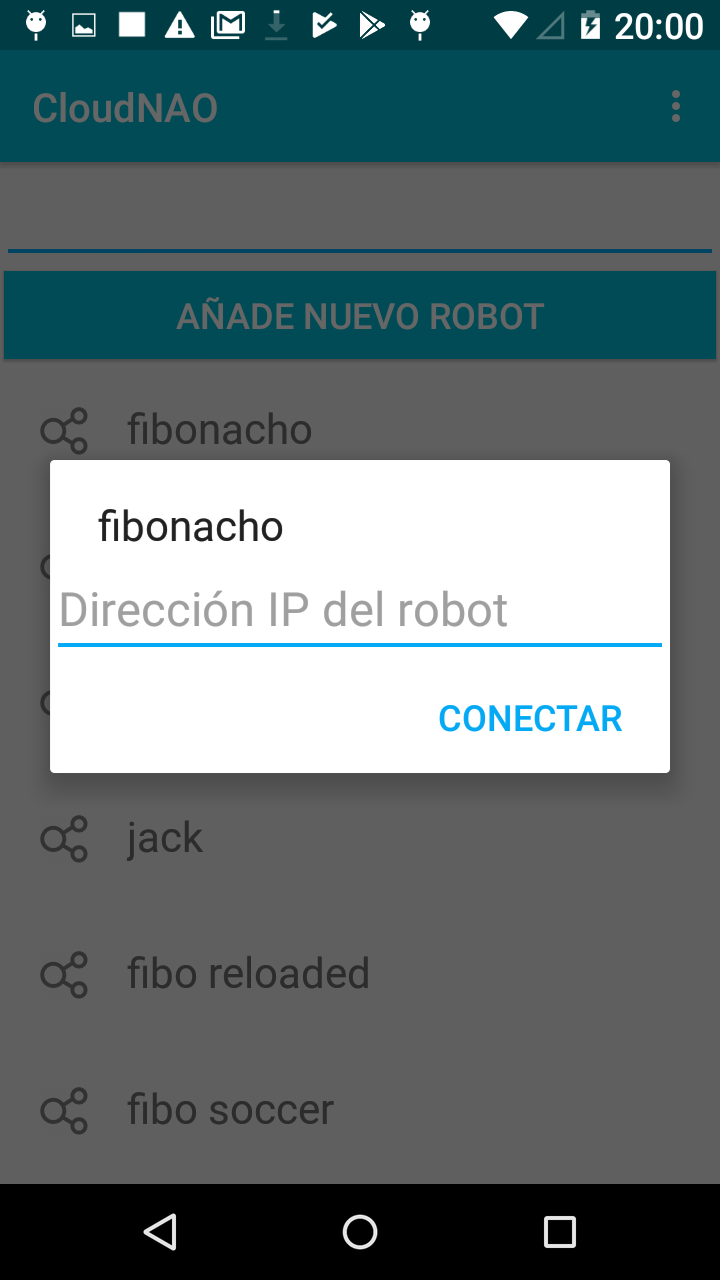
\includegraphics[scale=.1]{robot_connection_app1}}%
    \qquad
    \subfloat{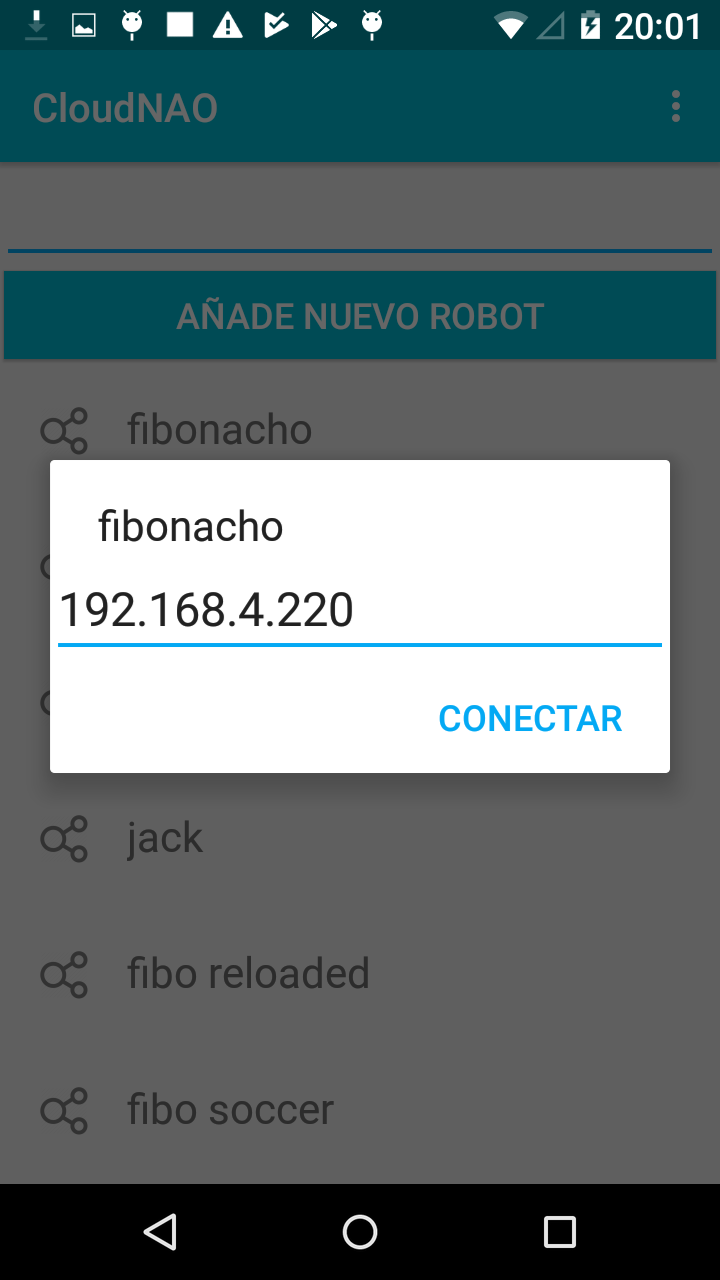
\includegraphics[scale=.1]{robot_connection_app2}}%
    \caption{Para conectarse con un robot simplemente se ingresa la dirección
    IP de éste.}
    
\end{figure}


\subparagraph{Menú intuitivo.}
Las actividades que se pueden realizar después de conectar
la aplicación con el robot se muestran en un menú intuitivo.

\begin{figure}[!h]
    \centering

    \subfloat{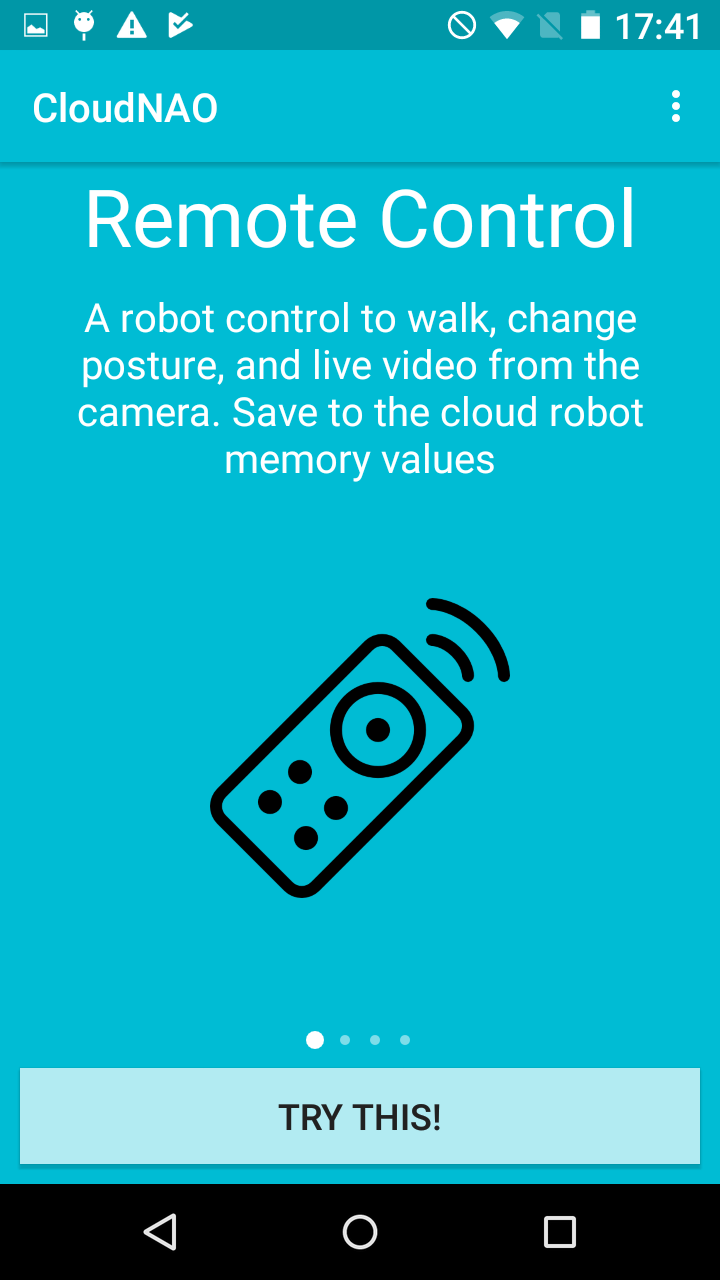
\includegraphics[scale=.09]{menu_rc}}%
    \qquad
    \subfloat{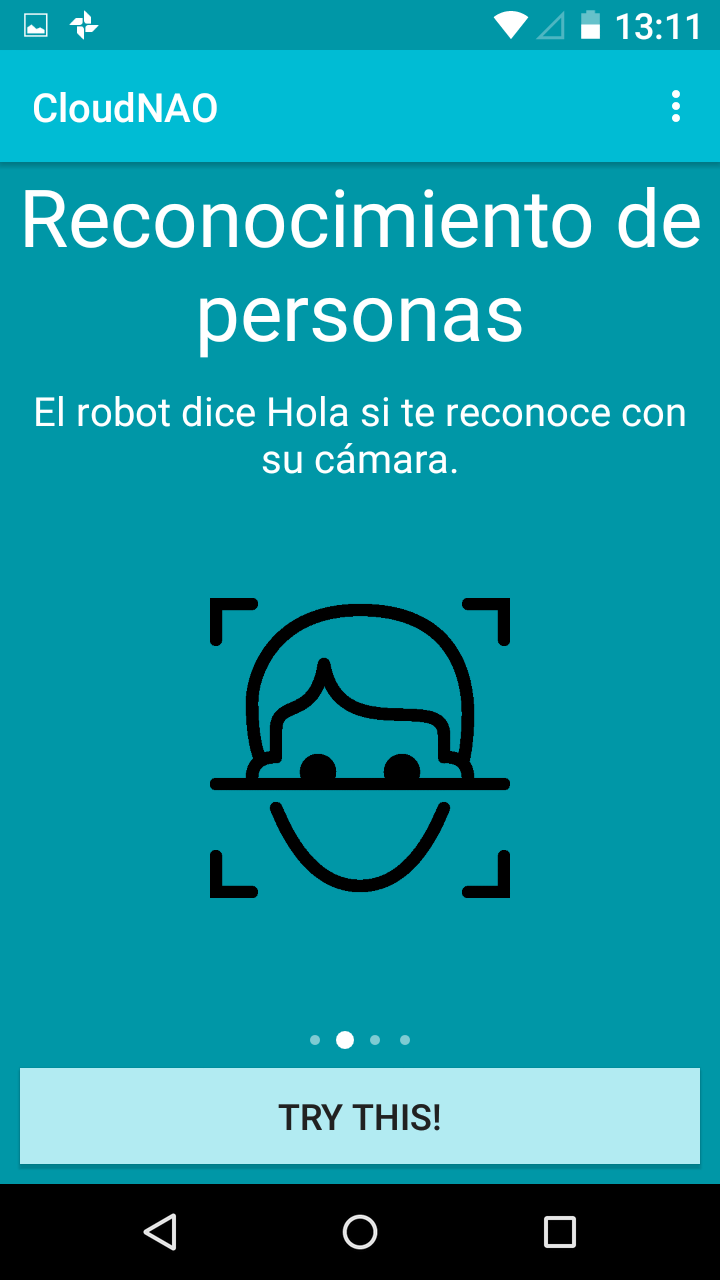
\includegraphics[scale=.09]{menu_face}}%
    \qquad
    \subfloat{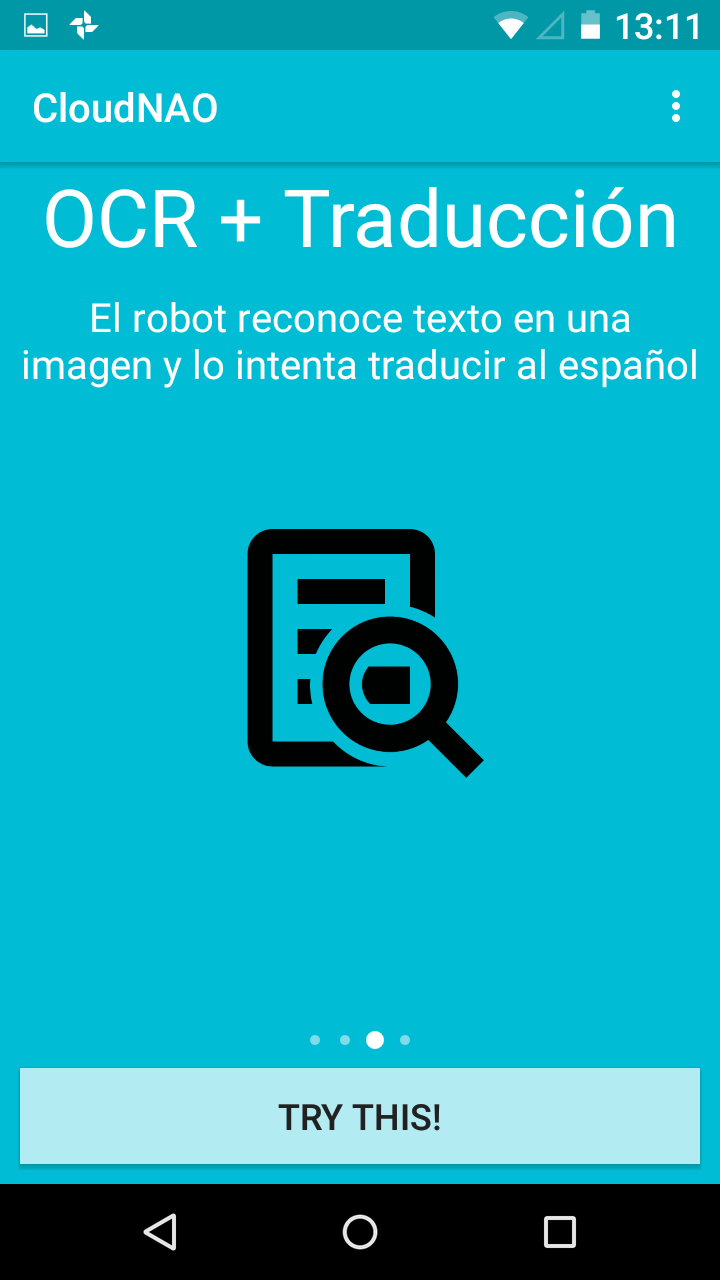
\includegraphics[scale=.09]{menu_ocr}}%
    \qquad
    \subfloat{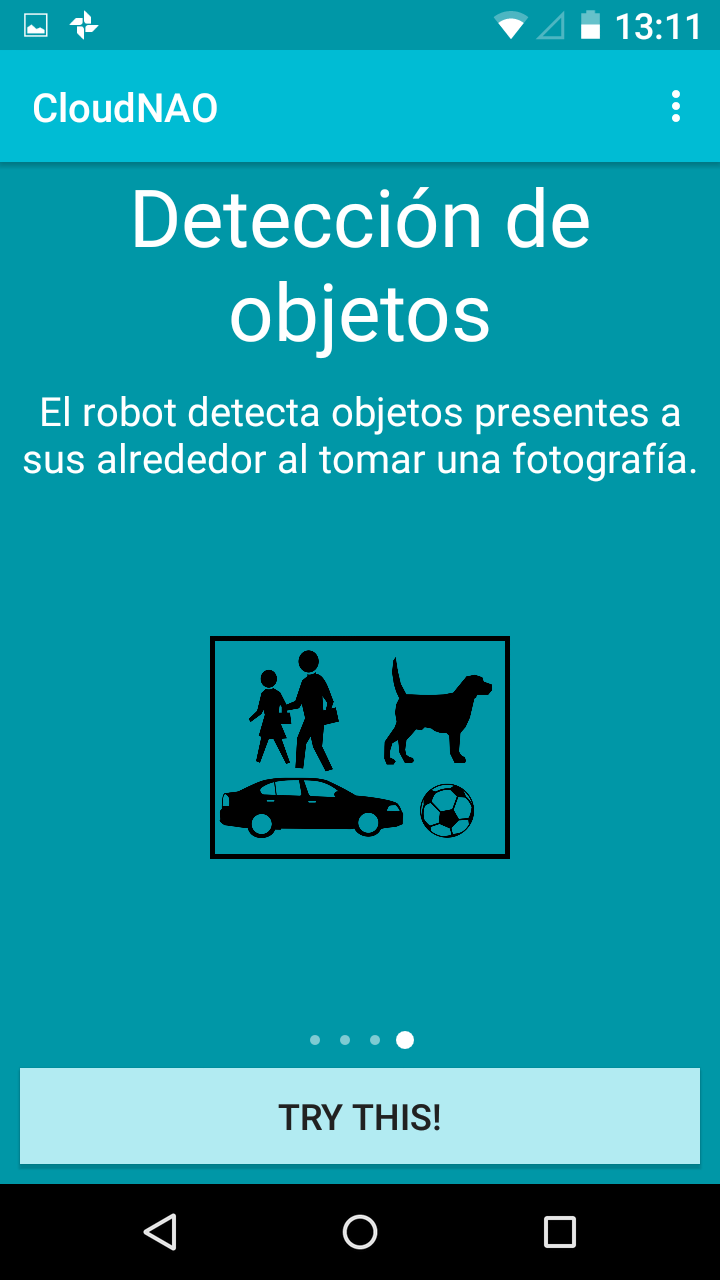
\includegraphics[scale=.09]{menu_objects}}%
    \caption{La pantallas del menú de la aplicación.}
\end{figure}



\subparagraph{Control remoto.}
\label{\detokenize{users_docs:control-remoto-para-el-robot}}
Una primera necesidad que se encontró y por la que surgió todo el proyecto
fue crear un control remoto para el robot NAO. Es muy básico pero admite
comandos para hacer al robot caminar sobre sus tres ejes y cambiar entre dos
posturas. El control remoto incluye una imagen en vivo de la
cámara del robot.

\begin{figure}[!h]
    \centering
	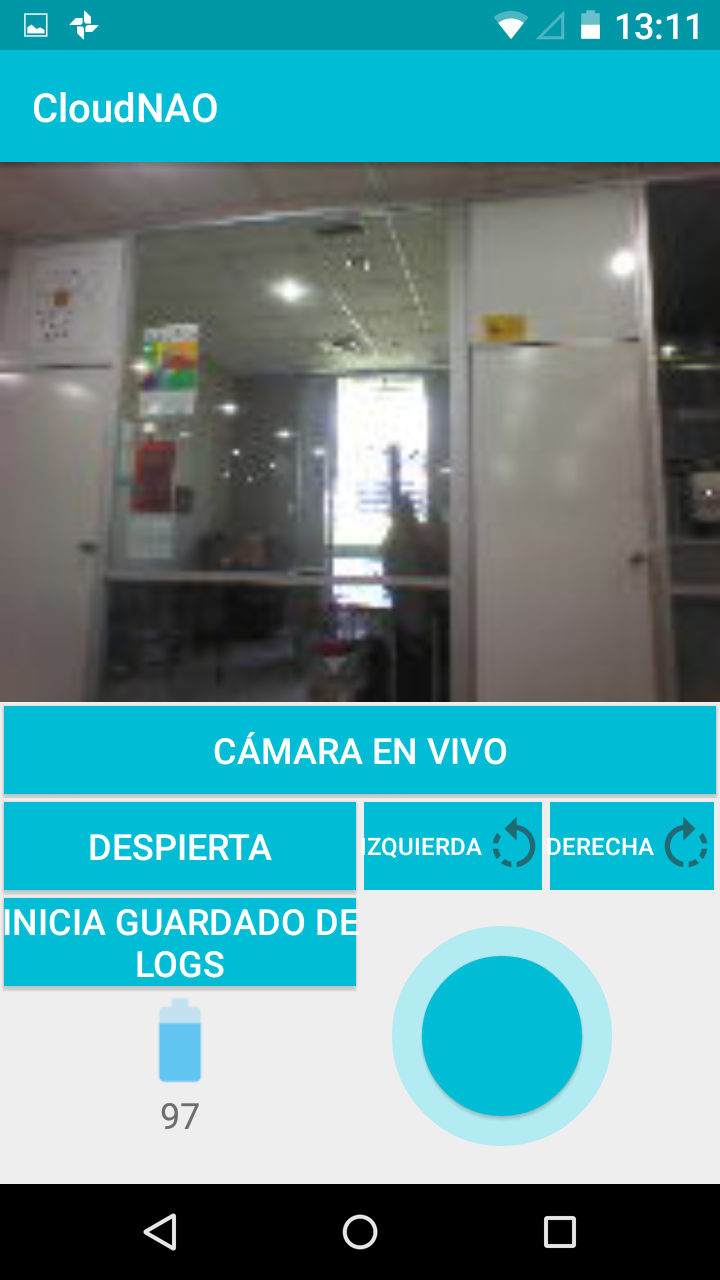
\includegraphics[scale=.1]{rc_image}
	\caption{El control remoto muestra una imagen en vivo si se desea, el estado del batería y un joystick para mover al robot.}
\end{figure}


\subparagraph{Guarda valores de ALMemory en la nube.}
\label{\detokenize{users_docs:guarda-valores-de-almemory-en-la-nube}}
Otra función dentro del control remoto es la de la opción de guardar ciertos
valores de la memoria del robot en la nube, para consultarlos o descargarlos
después en la aplicación web. El conjunto de valores que por ahora
están disponibles para su almacenamiento son los siguientes:
rightUSSensorValue, leftUSSensorValue, rightFootTotalWeight, RightBumperPressed, leftFootTotalWeight, ChestButtonPressed, RearTactilTouched, leftFootContact, LeftBumperPressed, footContact, FrontTactilTouched, BatteryChargeChanged, PostureChanged, rightFootContact, MiddleTactilTouched, GyrometerX, GyrometerY, AccelerometerX, AccelerometerY, AccelerometerZ, TorsoAngleX, TorsoAngleY.

\begin{figure}[!h]
    \centering
    \subfloat{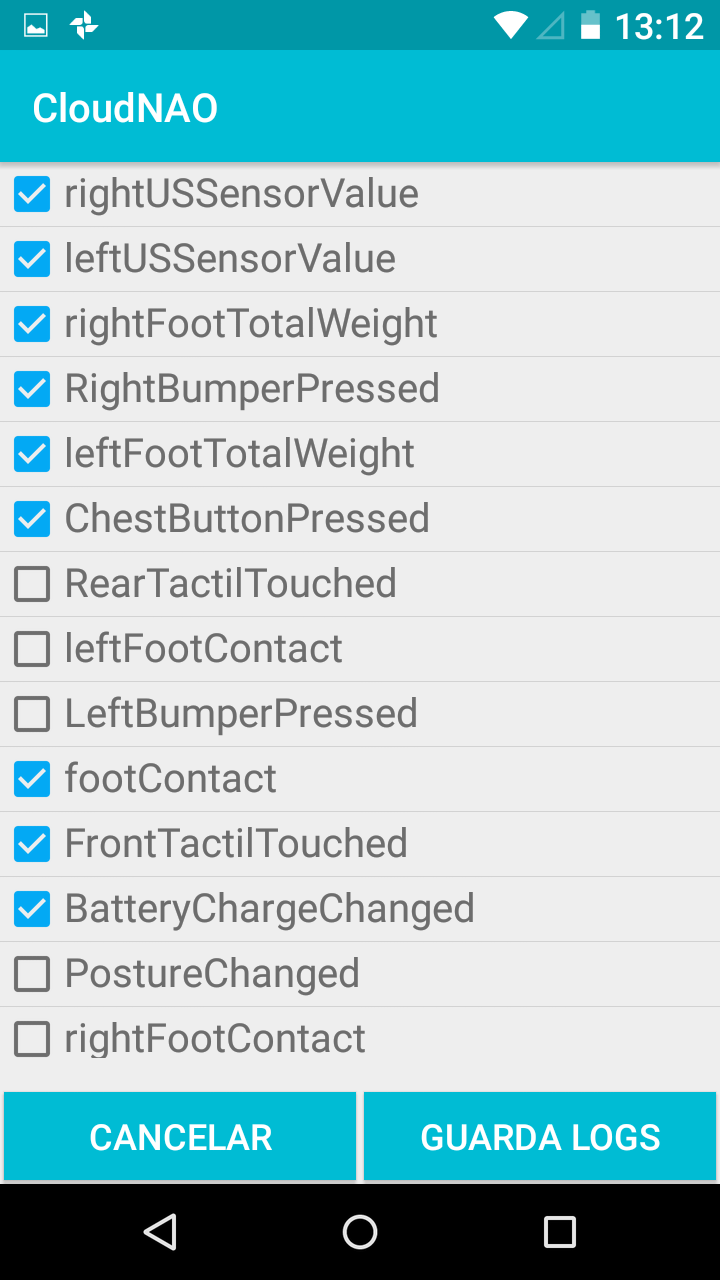
\includegraphics[scale=.1]{memory_list}}%
    \qquad
    \subfloat{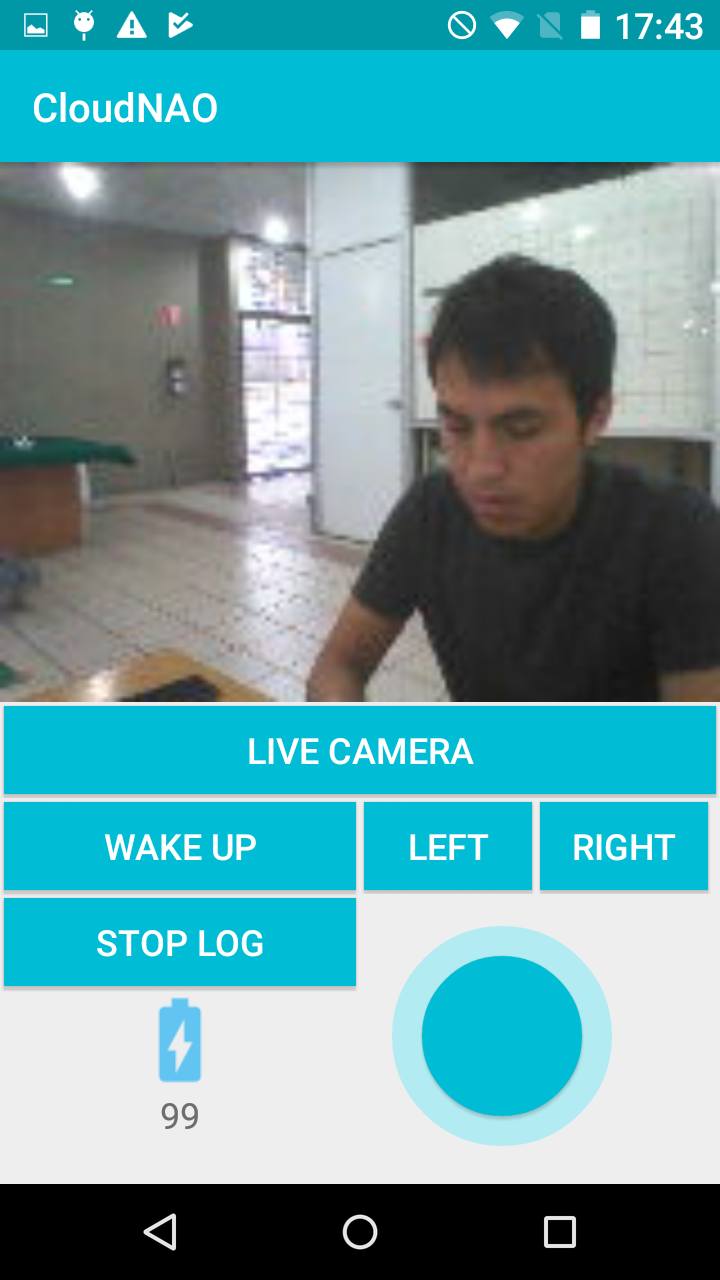
\includegraphics[scale=.1]{rc_image3}}
    \caption{Después de dar clic en el botón START LOG se abre una pantalla para elegir los valores de la memoria que se desean guardar
    en Firebase.}
\end{figure}


\subparagraph{Detección de rostros y reconocimiento de sujetos en una fotografía enviada por el robot.}
\label{\detokenize{users_docs:deteccion-de-rostros-en-una-fotografia-enviada-por-el-robot}}
Esta funcionalidad permite a un usuario
capturar una fotografía con la cámara del robot, añadir
una etiqueta a un rostro si fue encontrado y guardar esa cara para su futuro reconocimiento.
Cuando detecta a un sujeto previamente guardado el robot ejecuta 
un gesto de saludo.

\begin{figure}[!h]
    \centering
    
    \subfloat{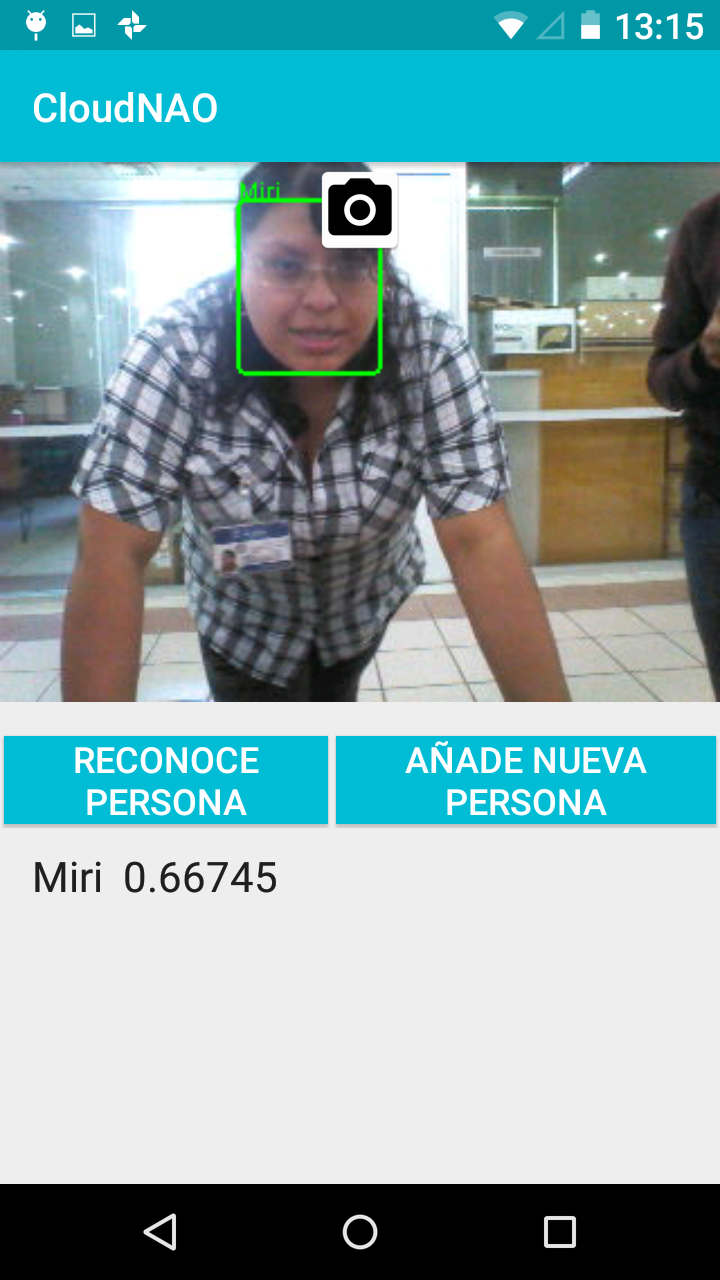
\includegraphics[scale=.1]{face}}%
\caption{Ejemplo de el reconocimiento de una persona que antes fue detectada.}
\end{figure}


\subparagraph{Detección de objectos de entre 80 categorías en una imagen de la cámara del robot.}
\label{\detokenize{users_docs:deteccion-de-objectos-de-entre-80-categorias-en-una-imagen-de-la-camara-del-robot}}
Funciona de manera similar a la detección de rostros. Envía una imagen capturada
con la cámara del robot a la API RESTful de CloudNAO, que ejecuta un módulo
con la API de detección de objectos de TensorFlow y se procesa la respuesta para
que en la pantalla se dibujen unos
recuadros delimitadores sobre los objectos detectados así como una etiqueta
con el nombre que le corresponde. El robot simplemente
dice la cantidad de objetos que ve de acuerdo a las categorías válidas.

\begin{figure}[!h]
    \centering
	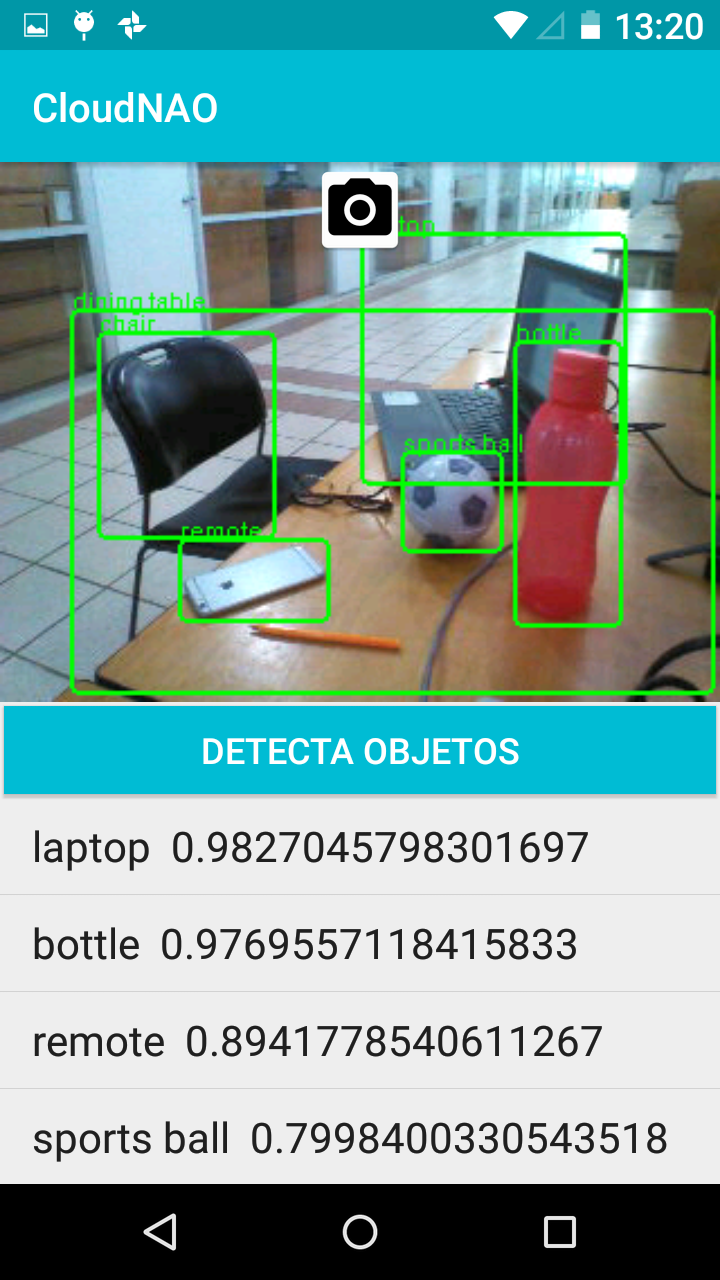
\includegraphics[scale=.1]{object}%
	\caption{Después de detectar los objetos el robot da una lista enumerada
	de éstos.}
\end{figure}


\subparagraph{Reconocimiento óptico de caracteres y traducción de texto encontrados en una imagen enviada por el robot.}
\label{\detokenize{users_docs:reconocimiento-optico-de-caracteres-y-traduccion-de-texto-encontrados-en-una-imagen-enviada-por-el-robot}}
La aplicación solicita una imagen del robot, esa imagen es parte de la petición
a la API RESTful de CloudNAO, igual que en las dos funcionalidades anteriores.
Se buscan caracteres dentro de la imagen, para su posterior traducción.
El resultado se muestra en dos partes, una es el texto original y el otro
es el texto traducido al español. El robot tiene la opción de convertir la
traducción en un discurso oral.

\begin{figure}[!h]
    \centering
    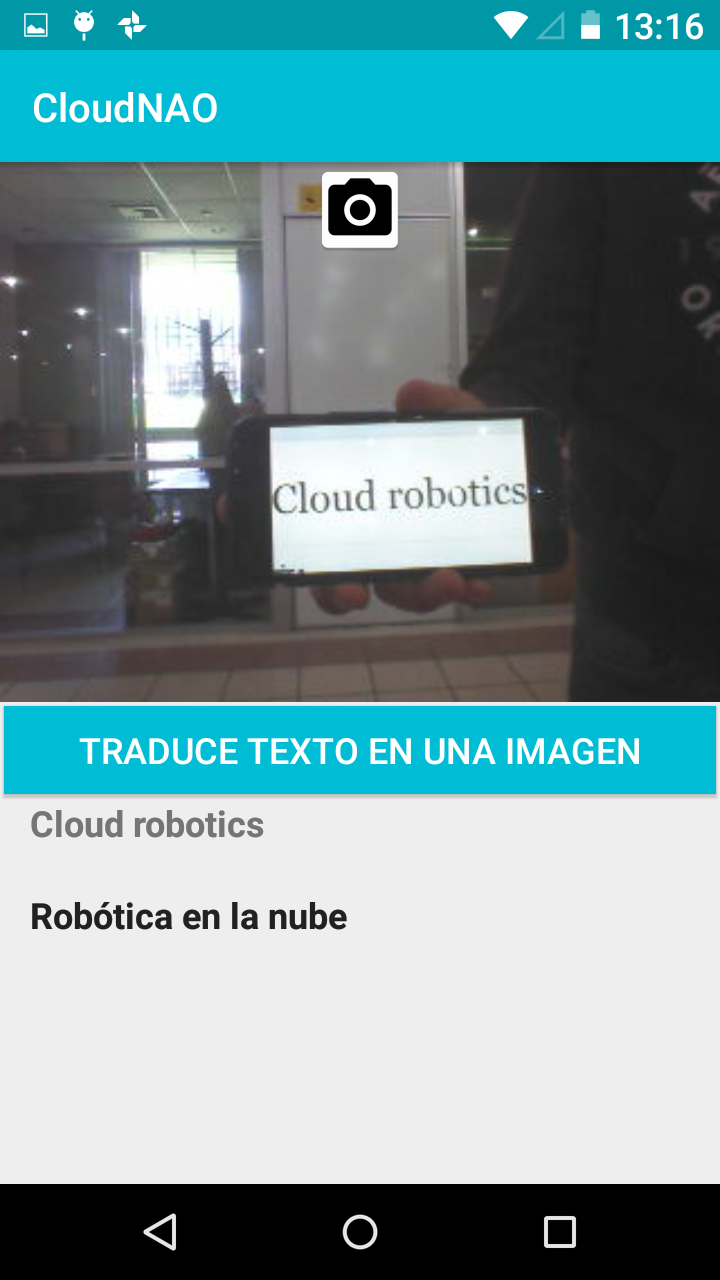
\includegraphics[scale=.1]{ocr_before}
    \caption{Al presionar el texto traducido el robot repite oralmente la cadena
    de caracteres.}
\end{figure}


% \subsubsection{Demostración de la aplicación funcionando}
% \label{\detokenize{users_docs:demostracion-de-la-aplicacion-funcionando}}
% En esta sección se describe de manera pictórica el flujo de la aplicación.
% Desde que el usuario inicia sesión, selecciona un robot y se conecta a él,
% y recorre cada una de las opciones del menú.

% Cada parte va acompañada de una captura de pantalla de la aplicación y
% una fotografía del robot si esta es necesaria.


% \paragraph{Inicio de sesión}
% \label{\detokenize{users_docs:inicio-de-sesion}}

% \paragraph{Selección de Robot}
% \label{\detokenize{users_docs:seleccion-de-robot}}

% \paragraph{Recorrido por el menú}
% \label{\detokenize{users_docs:recorrido-por-el-menu}}

% \paragraph{Control remoto}
% \label{\detokenize{users_docs:control-remoto}}

% \paragraph{Reconocimiento facial}
% \label{\detokenize{users_docs:reconocimiento-facial}}

% \paragraph{Reconocimiento óptico de caracteres y traducción}
% \label{\detokenize{users_docs:reconocimiento-optico-de-caracteres-y-traduccion}}

% \paragraph{Detección de objetos}
% \label{\detokenize{users_docs:deteccion-de-objetos}}

% \paragraph{Cierra la conexión con el robot}
% \label{\detokenize{users_docs:cierra-la-conexion-con-el-robot}}

% \paragraph{Cierra la sesión del usuario}
% \label{\detokenize{users_docs:cierra-la-sesion-del-usuario}}

\subsubsection{Guía para desarrolladores}
\label{\detokenize{dev_docs::doc}}\label{\detokenize{dev_docs:guia-para-desarrolladores}}

Para desarrollar la aplicación fueron tres los elementos importantes:
\begin{itemize}
\item {} 
Un entorno de desarrollo integrado (\textbf{Android Studio}).

\item {} 
El robot humanoide NAO (no simulado).

\item {} 
El SDK para Android de NAOqi.

\end{itemize}

Además de los elementos anteriores se necesitan una computadora y acceso a una red inalámbrica
en cada uno de los dispositivos.

En el Anexo \ref{anexo:app-android}
se describen las herramientas ocupadas durante 
el desarrollo de la aplicación:
Android Studio, Firebase Realtime
Database, Firebase UI para la autenticación, y las bibliotecas Butterknife
y Volley para el manejo de la IU y para las peticiones a la API REST,




% \subsection{referencias}
% \label{\detokenize{dev_docs:referencias}}
% \sphinxurl{https://developer.android.com/studio/intro/index.html?hl=es-419}
% \sphinxurl{https://medium.com/@petehouston/compile-local-jar-files-with-gradle-a078e5c7a520}
% \sphinxurl{https://github.com/firebase/FirebaseUI-Android/blob/master/auth/README.md}
% \sphinxurl{http://jakewharton.github.io/butterknife/}


\subsubsection{Descripción de las clases principales}
\label{\detokenize{dev_docs:documentacion-para-desarrolladores}}

La aplicación está compuesta como cualquier otra, por una
carpeta \textit{manifests}, \textit{res} y \textit{java}.
La carpeta \textit{java} incluye los paquetes \texttt{com.lar.cloudnao.utilities} y \texttt{com.lar.cloudnao}.


\paragraph{Paquete \texttt{utilities}}

Es un paquete compuesto por clases e interfaces que tienen como
función realizar tareas asíncronas para manejar imágenes del robot,
enviar peticiones a la API REST, manejar la IU, etcétera.\\

\codedocumentation{\texttt{Interface }\sphinxcode{OnRobotNameClickListener}}
Una interfaz con un método abstracto que sirve como callback
cuando un usuario da clic sobre alguno de los robots obtenidos desde Firebase y mostrados en un \texttt{RecyclerView}.
\newline

\codedocumentation{\texttt{Interface }\sphinxcode{VisionRequestCompleted}}
Interfaz con un método abstracto que se llama dentro de una tarea asíncrona para procesar un objeto que se obtiene de la respuesta
a la solicitud del recurso \texttt{vision} de la API REST de CloudNAO.
Hereda métodos de \texttt{AsyncTask}.
\newline

\codedocumentation{\texttt{Class }\sphinxcode{BatteryStatusTask}}
Esta clase obtiene el nivel de batería actual en el robot a través de la lectura del valor en 
\texttt{ALMemory}. Utiliza la clase \texttt{AsyncTask}.
Muestra una \texttt{ImageView} que representa el estado de la batería y un \texttt{TextView} con el porcentaje de batería restante.
\newline

\codedocumentation{\texttt{Class }\sphinxcode{BoundingBoxesUtils}}
Una clase estática con un método para dibujar cuadros delimitadores 
sobre un \texttt{ImageView}. Para dibujar el cuadro delimitador 
recibe un arreglo con los valores necesarios para generar las 
coordenadas que se usan para dibujar.
\newline

\codedocumentation{\texttt{Class }\sphinxcode{ImageTask}}
Clase pública con métodos asíncronos para obtener una imagen desde la cámara del robot de manera remota.  Obtiene un objeto que contiene la imagen, con el espacio de color por defecto del robot NAO (YUV) en un arreglo de bytes, convierte ese arreglo en una imagen jpeg, para después cargar ese objeto jpeg en un bitmap que sirve para llenar el \texttt{ImageView} que muestra la imagen enviada por el robot. Es una subclase
de \texttt{AsyncTask}.
\newline

\codedocumentation{\texttt{Class }\sphinxcode{ItemsListAdapter}}
Esta clase es el \texttt{Adapter} para el \texttt{ListView} cuyos elementos 
están compuestos por un \texttt{CheckBox} y un \texttt{TextView}. Se 
utiliza al mostrar la lista de datos que se quieren guardar en 
Firebase desde \texttt{ALMemory}.
\newline

\codedocumentation{\texttt{Class }\sphinxcode{MyPagerAdapter}}
Subclase de \texttt{PagerAdapter} para el \texttt{ViewPager} del menú
principal de la aplicación, por ahora tiene un tamaño máximo de 4. 
\newline

\codedocumentation{\texttt{Class }\sphinxcode{ProxySubscriberItem}}
Clase pública para modelar los objetos de la lista con los datos de \texttt{ALMemory} que se guardarán en Firebase. \texttt{ItemsListAdapter} contiene un objeto \texttt{List} de
instancias de \texttt{ProxySu	bscriberItem}. Los
atributos son un  valor booleano \texttt{mChecked} y una cadena \texttt{mProxyName} para saber si un ítem está marcado y el nombre
de la llave en \texttt{ALMemory}, respectivamente.
\newline

\codedocumentation{\texttt{Class }\sphinxcode{RecyclerViewAdapter}}
La clase pública del \texttt{Adapter} para el \texttt{RecyclerView} que mostrará la lista de robots obtenidos desde Firebase y que le pertenecen al
usuario que inició sesión en la aplicación.
\newline

\codedocumentation{\texttt{Class }\sphinxcode{RecyclerViewHolders}}
La clase que modela a los \texttt{ViewHolders} que representan cada robot obtenido de Firebase.
Aquí se utiliza el método abstracto \texttt{onClickRobotName} como callback para ejecutar una acción al dar clic sobre un elemento del \texttt{RecyclerView}.
\newline

\codedocumentation{\texttt{Class }\sphinxcode{RobotFromFirebase}}
La clase que modela los objetos de la lista de robots obtenidos desde Firebase, cada objeto contiene un identificador único y el nombre que el usuario asignó.
\newline

\codedocumentation{\texttt{Class }\sphinxcode{RobotLogs}}
Clase con métodos asíncronos para almacenar valores de \texttt{ALMemory} en Firebase, obtiene valores del robot y los almacena en una ubicación en Firebase con un \texttt{push()}, por lo que se genera un historial de logs.
\newline

\codedocumentation{\texttt{Class }\sphinxcode{ViewHolder}}
Clase que modelos los \texttt{ViewHolders} de la lista de datos que se desean guardar en Firebase, están compuestos por un \texttt{CheckBox} y un \texttt{TextView} que describe a cada elemento.
\newline

\codedocumentation{\texttt{Class }\sphinxcode{VisionListElement}}
Clase pública que modela los objetos dentro de una lista que muestra resultados de las actividades de reconocimiento de rostros y objetos. Cada instancia tiene un identificador, que puede ser el nombre del sujeto reconocido , la confianza y las coordenadas de que delimitan al elemento encontrado (un cuadro que encierra un rostro, o un rectángulo que acota un objeto).
\newline

\codedocumentation{\texttt{Class }\sphinxcode{VisionRESTRequestsTask}}
La clase con métodos asíncronos para hacer peticiones a la API REST 
de CloudNAO. Recibe la imagen desde un \texttt{ImageView}, del que obtiene un 
bitmap y genera una cadena en base 64 que representa esa imagen. 
Después define la estructura y valores del JSON que se envía en una 
petición usando la biblioteca Volley. A partir de la respuesta 
obtenida ejecuta la función callback \texttt{onVisionRequestCompleted} 
para mostrar los resultados en el contexto de donde se solicitó.
\newline

\codedocumentation{\texttt{Class }\sphinxcode{VolleyResponseUtils}}
Clase estática para manejar la repuesta de \texttt{Volley}, que puede ser un error o puede ser la estructura que se espera.
\newline

\codedocumentation{\texttt{Enum ModelObjectViewPager}}
Un enumerado de Java que representa todas las posibles páginas del ViewPager. Se utiliza en el menú de la aplicación. En este enumerado se almacenan el identificador del \texttt{Layout} de cada página y un título que le corresponde.


\paragraph{Actividades de la aplicación}

\codedocumentation{\texttt{Class FaceRecognitionActivity}}
La clase de la actividad que realiza el reconocimiento de rostros. Implementa la interfaz \texttt{VisionRequestCompleted} para llamar a su método abstracto desde la clase \texttt{VisionRESTRequestsTask}.
\newline

\codedocumentation{\texttt{Class MenuActivity}}
La actividad que muestra el menú principal donde se elige entre otras actividades para interactuar con el robot. Muestra un \texttt{ViewPager} para navegar y elegir la actividad deseada.
\newline

\codedocumentation{\texttt{Class ObjectDetectionActivity}}
La actividad encargada de la funcionalidad de la detección de objetos, implementa la interfaz \texttt{VisionRequestCompleted} para ejecutar su método \texttt{VisionRequest\\Completed.onVisionRequestComple\\ted(Object)} como callback en \texttt{VisionRESTRequestsTask}.


\codedocumentation{\texttt{Class OCRTranslationActivity}}
Clase de la actividad que se encarga del procesamiento de una imagen 
para detección de texto y su traducción. Implementa la interfaz 
\texttt{VisionRequestCompleted}.
\newline

\codedocumentation{\texttt{Class RemoteControllerActivity}}
La actividad para el control remoto del robot. Además de poder 
controlar algunos movimientos como el caminado o el cambio de postura, 
se puede visualizar una imagen en vivo de la cámara del robot, así 
como permite enviar valores de \texttt{ALMemory} a una base de datos en la nube 
a través de Firebase.
\newline

\codedocumentation{\texttt{Class Robot}}
No es una actividad pero es la clase pública principal para ejecutar módulos del framework de NAOqi en la aplicación. Es una interfaz para conectarse al robot y ejecutar algunos módulos de NAOqi. Usa el patrón de diseño Singleton para que solo exista una instancia del objeto y funcione como una variable global.
\newline

\codedocumentation{\texttt{Class SelectRobotActivity}}
Actividad que muestra los robots registrados por el usuario así como la opción para añadir nuevos robots, o conectarse a uno de la lista. Implementa el método abstracto \texttt{OnRobotNameClickListener.onClickRobotName(String, String)}.

%
%\begin{itemize}
%\item {} 
%\sphinxcode{SignInActivity}, la actividad encargada de todo el flujo para el inicio de sesión. Utiliza FirebaseUI.
%
%\item {} 
%\sphinxcode{SelectRobotActivity}, la actividad que muestra los robots guardados por el usuario que inició sesión. Además aquí se pueden añadir nuevos. Escribe y lee de Firebase Realtime Database. Aquí se crea la instancia única del robot con el que se desea conectar, se crea la sesión y los proxies a los módulos de NAOqi.
%
%\item {} 
%\sphinxcode{MenuActivity}, esta actividad es un menú para elegir entre las actividades restantes. Es un ViewPager, que reacciona al click del usuario.
%
%\item {} 
%\sphinxcode{RemoteControllerActivity}, la actividad que corresponde al control remoto. Utiliza módulos de NAOqi, y la base de datos de Firebase para escribir los logs.
%
%\item {} 
%\sphinxcode{FaceRecognitionActivity}, la actividad que detecta rostros en una imagen. Utiliza Volley para conectarse a la API RESTful de CloudNAO.
%
%\item {} 
%\sphinxcode{OCRTranslationActivity}, esta actividad reconoce texto en una imagen y lo traduce. Utiliza Volley para conectarse a la API RESTful de CloudNAO.
%
%\item {} 
%\sphinxcode{ObjectDetectionActivity}, la actividad que reconoce objetos en una imagen. Utiliza Volley para conectarse a la API RESTful de CloudNAO.
%
%\item {} 
%\sphinxcode{Robot}, es la clase que define al objeto robot. Los métodos para ejecutar módulos de NAOqi, y obtener imágenes de la cámara del robot, valores de la memoria, etc.
%
%\end{itemize}


% \textbf{SignInActivity}
% \label{\detokenize{dev_docs:signinactivity}}\index{SignInActivity (Java class)}

% \begin{fulllineitems}
% \phantomsection\label{\detokenize{dev_docs:com.lar.cloudnao.SignInActivity}}\pysigline{public class \sphinxbfcode{SignInActivity} extends AppCompatActivity}
% La actividad para iniciar sesión en la aplicación, utiliza la biblioteca Firebae UI, para facilitar el flujo del inicio de sesión.

% \end{fulllineitems}



% \textbf{Métodos}
% \label{\detokenize{dev_docs:methods}}

% \textbf{OnClickSignInButton}
% \label{\detokenize{dev_docs:onclicksigninbutton}}\index{OnClickSignInButton() (Java method)}

% \begin{fulllineitems}
% \phantomsection\label{\detokenize{dev_docs:com.lar.cloudnao.SignInActivity.OnClickSignInButton()}}\pysiglinewithargsret{public void \sphinxbfcode{OnClickSignInButton}}{}{}
% Agrega un escuchador al botón signInButton para crear un intent sign-in. Este intent es provisto por la biblioteca de Firebase AuthUI. Esto construye una actividad sign-in, y pasa un entero RC\_SIGN\_IN, que es una variable donde se guarda la respuesta de la actividad sign-in. Cuando esa actividad finaliza su trabajo enviará de regreso onActivityResult que contiene el código de petición y otra información. Esa información es un intent, que podemos usar para descifrar que pasó.

% \end{fulllineitems}



% \textbf{createIntent}
% \label{\detokenize{dev_docs:createintent}}\index{createIntent(Context) (Java method)}

% \begin{fulllineitems}
% \phantomsection\label{\detokenize{dev_docs:com.lar.cloudnao.SignInActivity.createIntent(Context)}}\pysiglinewithargsret{public static Intent \sphinxbfcode{createIntent}}{Context\sphinxstyleemphasis{ context}}{}
% Este método se utiliza por la actividad sign-in en caso de que no se tenga un usuario válido.

% \end{fulllineitems}



% \textbf{onActivityResult}
% \label{\detokenize{dev_docs:onactivityresult}}\index{onActivityResult(int, int, Intent) (Java method)}

% \begin{fulllineitems}
% \phantomsection\label{\detokenize{dev_docs:com.lar.cloudnao.SignInActivity.onActivityResult(int, int, Intent)}}\pysiglinewithargsret{protected void \sphinxbfcode{onActivityResult}}{int\sphinxstyleemphasis{ requestCode}, int\sphinxstyleemphasis{ resultCode}, Intent\sphinxstyleemphasis{ data}}{}
% Verifica y maneja el resultado enviado por la actividad sign-in

% \end{fulllineitems}



% \textbf{onCreate}
% \label{\detokenize{dev_docs:oncreate}}\index{onCreate(Bundle) (Java method)}

% \begin{fulllineitems}
% \phantomsection\label{\detokenize{dev_docs:com.lar.cloudnao.SignInActivity.onCreate(Bundle)}}\pysiglinewithargsret{protected void \sphinxbfcode{onCreate}}{Bundle\sphinxstyleemphasis{ savedInstanceState}}{}
% Es el método que se llama al crear la actividad, si el usuario ya ha iniciado sesión ejecuta la actividad de la clase SelectRobotActivity y finaliza la actual.

% \end{fulllineitems}



% \textbf{SelectRobotActivity}
% \label{\detokenize{dev_docs:selectrobotactivity}}\index{SelectRobotActivity (Java class)}

% \begin{fulllineitems}
% \phantomsection\label{\detokenize{dev_docs:com.lar.cloudnao.SelectRobotActivity}}\pysigline{public class \sphinxbfcode{SelectRobotActivity} extends AppCompatActivity implements OnRobotNameClickListener}
% Actividad que muestra los robots registrados por el usuario así como la opción para añadir nuevos robots, o conectarse a uno de la lista. Implementa el método abstracto \sphinxcode{OnRobotNameClickListeneronClickRobotName(String,String)}.

% \end{fulllineitems}



% \subsubsection{Atributos}
% \label{\detokenize{dev_docs:fields}}

% \paragraph{MyRobot}
% \label{\detokenize{dev_docs:myrobot}}\index{MyRobot (Java field)}

% \begin{fulllineitems}
% \phantomsection\label{\detokenize{dev_docs:com.lar.cloudnao.SelectRobotActivity.MyRobot}}\pysigline{public {\hyperref[\detokenize{dev_docs:com.lar.cloudnao.Robot}]{\sphinxcrossref{Robot}}} \sphinxbfcode{MyRobot}}
% Llama a las instancia global de {\hyperref[\detokenize{dev_docs:com.lar.cloudnao.Robot}]{\sphinxcrossref{\sphinxcode{Robot}}}}

% \end{fulllineitems}



% \paragraph{mNewRobotEditText}
% \label{\detokenize{dev_docs:mnewrobotedittext}}\index{mNewRobotEditText (Java field)}

% \begin{fulllineitems}
% \phantomsection\label{\detokenize{dev_docs:com.lar.cloudnao.SelectRobotActivity.mNewRobotEditText}}\pysigline{ EditText \sphinxbfcode{mNewRobotEditText}}
% Campo para añadir el nombre de un nuevo robot.

% \end{fulllineitems}



% \paragraph{robotListFromFirebaseRecyclerView}
% \label{\detokenize{dev_docs:robotlistfromfirebaserecyclerview}}\index{robotListFromFirebaseRecyclerView (Java field)}

% \begin{fulllineitems}
% \phantomsection\label{\detokenize{dev_docs:com.lar.cloudnao.SelectRobotActivity.robotListFromFirebaseRecyclerView}}\pysigline{ RecyclerView \sphinxbfcode{robotListFromFirebaseRecyclerView}}
% La lista de los robots del usuario, se llena desde Firebase.

% \end{fulllineitems}



% \subsubsection{Métodos}
% \label{\detokenize{dev_docs:id3}}

% \paragraph{addNewRobot}
% \label{\detokenize{dev_docs:addnewrobot}}\index{addNewRobot() (Java method)}

% \begin{fulllineitems}
% \phantomsection\label{\detokenize{dev_docs:com.lar.cloudnao.SelectRobotActivity.addNewRobot()}}\pysiglinewithargsret{public void \sphinxbfcode{addNewRobot}}{}{}
% Escuchador para el botón que permite a los usuarios añadir un nuevo robot.

% \end{fulllineitems}



% \paragraph{onClickRobotName}
% \label{\detokenize{dev_docs:onclickrobotname}}\index{onClickRobotName(String, String) (Java method)}

% \begin{fulllineitems}
% \phantomsection\label{\detokenize{dev_docs:com.lar.cloudnao.SelectRobotActivity.onClickRobotName(String, String)}}\pysiglinewithargsret{public void \sphinxbfcode{onClickRobotName}}{\sphinxhref{http://docs.oracle.com/javase/8/docs/api/java/lang/String.html}{String}\sphinxstyleemphasis{ robotName}, \sphinxhref{http://docs.oracle.com/javase/8/docs/api/java/lang/String.html}{String}\sphinxstyleemphasis{ robotUID}}{}
% Define al método abstracto \sphinxcode{OnRobotNameClickListeneronClickRobotName(String,String)} para servir como callback cuando un usuario da clcik en un robot de la lista. Muestra un cuadro de diálogo con TextView para agregar la dirección IP del robot y ejecutar \sphinxcode{ConnectionTask}.

% \end{fulllineitems}



% \paragraph{onCreate}
% \label{\detokenize{dev_docs:id4}}\index{onCreate(Bundle) (Java method)}

% \begin{fulllineitems}
% \phantomsection\label{\detokenize{dev_docs:com.lar.cloudnao.SelectRobotActivity.onCreate(Bundle)}}\pysiglinewithargsret{protected void \sphinxbfcode{onCreate}}{Bundle\sphinxstyleemphasis{ savedInstanceState}}{}
% Inicia la actividad, verifica que el usuario haya iniciado sesión. Si el usuario es nuevo, entonces se añade a la ubicación /users en la base de datos de Firebase. Luego, agrega un escuchador a la ubicación de la base de datos que contiene a los robots del usuario. Llama al método \sphinxcode{getRobotFirebaseDataSnapshot()} para actualizar {\hyperref[\detokenize{dev_docs:com.lar.cloudnao.SelectRobotActivity.robotListFromFirebaseRecyclerView}]{\sphinxcrossref{\sphinxcode{robotListFromFirebaseRecyclerView}}}}.

% \end{fulllineitems}



% \paragraph{onCreateOptionsMenu}
% \label{\detokenize{dev_docs:oncreateoptionsmenu}}\index{onCreateOptionsMenu(Menu) (Java method)}

% \begin{fulllineitems}
% \phantomsection\label{\detokenize{dev_docs:com.lar.cloudnao.SelectRobotActivity.onCreateOptionsMenu(Menu)}}\pysiglinewithargsret{public boolean \sphinxbfcode{onCreateOptionsMenu}}{Menu\sphinxstyleemphasis{ menu}}{}
% Crea un menú de opciones para que por ahora contiene un elemento, cerrar la sesión del usuario.

% \end{fulllineitems}



% \paragraph{onOptionsItemSelected}
% \label{\detokenize{dev_docs:onoptionsitemselected}}\index{onOptionsItemSelected(MenuItem) (Java method)}

% \begin{fulllineitems}
% \phantomsection\label{\detokenize{dev_docs:com.lar.cloudnao.SelectRobotActivity.onOptionsItemSelected(MenuItem)}}\pysiglinewithargsret{public boolean \sphinxbfcode{onOptionsItemSelected}}{MenuItem\sphinxstyleemphasis{ item}}{}
% Añade un escuchador para cuando se selecciona un elemento en el menú de opciones. Por ahora solo cerrar sesión. Llama al método {\hyperref[\detokenize{dev_docs:com.lar.cloudnao.SelectRobotActivity.signOut()}]{\sphinxcrossref{\sphinxcode{signOut()}}}}.

% \end{fulllineitems}



% \paragraph{signOut}
% \label{\detokenize{dev_docs:signout}}\index{signOut() (Java method)}

% \begin{fulllineitems}
% \phantomsection\label{\detokenize{dev_docs:com.lar.cloudnao.SelectRobotActivity.signOut()}}\pysiglinewithargsret{public void \sphinxbfcode{signOut}}{}{}
% Cierra la sesión através de la biblioteca AuthUI

% \end{fulllineitems}



% \textbf{MenuActivity}
% \label{\detokenize{dev_docs:menuactivity}}\index{MenuActivity (Java class)}

% \begin{fulllineitems}
% \phantomsection\label{\detokenize{dev_docs:com.lar.cloudnao.MenuActivity}}\pysigline{public class \sphinxbfcode{MenuActivity} extends AppCompatActivity}
% La actividad que muestra el menú donde se elige entre otras actividades para interactuar con el robot. Muestra un ViewPager para navegar y elegir la actividad deseada.

% \end{fulllineitems}



% \subsubsection{Atributos}
% \label{\detokenize{dev_docs:id5}}

% \paragraph{MyRobot}
% \label{\detokenize{dev_docs:id6}}\index{MyRobot (Java field)}

% \begin{fulllineitems}
% \phantomsection\label{\detokenize{dev_docs:com.lar.cloudnao.MenuActivity.MyRobot}}\pysigline{public {\hyperref[\detokenize{dev_docs:com.lar.cloudnao.Robot}]{\sphinxcrossref{Robot}}} \sphinxbfcode{MyRobot}}
% La instancia del singleton de la clase {\hyperref[\detokenize{dev_docs:com.lar.cloudnao.Robot}]{\sphinxcrossref{\sphinxcode{Robot}}}}

% \end{fulllineitems}



% \paragraph{mCurrentPageSelected}
% \label{\detokenize{dev_docs:mcurrentpageselected}}\index{mCurrentPageSelected (Java field)}

% \begin{fulllineitems}
% \phantomsection\label{\detokenize{dev_docs:com.lar.cloudnao.MenuActivity.mCurrentPageSelected}}\pysigline{public int \sphinxbfcode{mCurrentPageSelected}}
% Un número que identifica la página que se muestra actualmente.

% \end{fulllineitems}



% \subsubsection{Métodos}
% \label{\detokenize{dev_docs:id7}}

% \paragraph{onClickMenuButton}
% \label{\detokenize{dev_docs:onclickmenubutton}}\index{onClickMenuButton() (Java method)}

% \begin{fulllineitems}
% \phantomsection\label{\detokenize{dev_docs:com.lar.cloudnao.MenuActivity.onClickMenuButton()}}\pysiglinewithargsret{public void \sphinxbfcode{onClickMenuButton}}{}{}
% Define el escuchador para el botón de selección de actividad dentro del menú de actividades.

% \end{fulllineitems}



% \paragraph{onCreate}
% \label{\detokenize{dev_docs:id8}}\index{onCreate(Bundle) (Java method)}

% \begin{fulllineitems}
% \phantomsection\label{\detokenize{dev_docs:com.lar.cloudnao.MenuActivity.onCreate(Bundle)}}\pysiglinewithargsret{protected void \sphinxbfcode{onCreate}}{Bundle\sphinxstyleemphasis{ savedInstanceState}}{}
% Inicializa la actividad, el ViewPager y el Adapter para escuchar cuando se cambia de página.

% \end{fulllineitems}



% \paragraph{onCreateOptionsMenu}
% \label{\detokenize{dev_docs:id9}}\index{onCreateOptionsMenu(Menu) (Java method)}

% \begin{fulllineitems}
% \phantomsection\label{\detokenize{dev_docs:com.lar.cloudnao.MenuActivity.onCreateOptionsMenu(Menu)}}\pysiglinewithargsret{public boolean \sphinxbfcode{onCreateOptionsMenu}}{Menu\sphinxstyleemphasis{ menu}}{}
% Crea un menú de opciones, en la barra superior y contar con una opción para desconectarse del robot (cerrando la sesión de NAOqi)

% \end{fulllineitems}



% \paragraph{onOptionsItemSelected}
% \label{\detokenize{dev_docs:id10}}\index{onOptionsItemSelected(MenuItem) (Java method)}

% \begin{fulllineitems}
% \phantomsection\label{\detokenize{dev_docs:com.lar.cloudnao.MenuActivity.onOptionsItemSelected(MenuItem)}}\pysiglinewithargsret{public boolean \sphinxbfcode{onOptionsItemSelected}}{MenuItem\sphinxstyleemphasis{ item}}{}
% Ejecuta la función \sphinxcode{closeRobotConnection()} si se selecciona la opción de desconectarse del robot desde el menú de opciones.

% \end{fulllineitems}



% \paragraph{startOCRActivity}
% \label{\detokenize{dev_docs:startocractivity}}\index{startOCRActivity() (Java method)}

% \begin{fulllineitems}
% \phantomsection\label{\detokenize{dev_docs:com.lar.cloudnao.MenuActivity.startOCRActivity()}}\pysiglinewithargsret{public void \sphinxbfcode{startOCRActivity}}{}{}
% Inicia la actividad {\hyperref[\detokenize{dev_docs:com.lar.cloudnao.OCRTranslationActivity}]{\sphinxcrossref{\sphinxcode{OCRTranslationActivity}}}}

% \end{fulllineitems}



% \paragraph{startObjectDetectionActivity}
% \label{\detokenize{dev_docs:startobjectdetectionactivity}}\index{startObjectDetectionActivity() (Java method)}

% \begin{fulllineitems}
% \phantomsection\label{\detokenize{dev_docs:com.lar.cloudnao.MenuActivity.startObjectDetectionActivity()}}\pysiglinewithargsret{public void \sphinxbfcode{startObjectDetectionActivity}}{}{}
% Inicia la actividad {\hyperref[\detokenize{dev_docs:com.lar.cloudnao.ObjectDetectionActivity}]{\sphinxcrossref{\sphinxcode{ObjectDetectionActivity}}}}

% \end{fulllineitems}



% \textbf{RemoteControllerActivity}
% \label{\detokenize{dev_docs:remotecontrolleractivity}}\index{RemoteControllerActivity (Java class)}

% \begin{fulllineitems}
% \phantomsection\label{\detokenize{dev_docs:com.lar.cloudnao.RemoteControllerActivity}}\pysigline{public class \sphinxbfcode{RemoteControllerActivity} extends AppCompatActivity}
% La actividad para el control remoto del robot. Además de poder controlar algunos movimientos como el caminado o el cambio de postura, se puede visualizar una imagen en vivo de la cámara del robot, así como permite enviar valores de ALMemory a una base de datos en la nube a través de Firebase.

% \end{fulllineitems}



% \subsubsection{Atributos}
% \label{\detokenize{dev_docs:id11}}

% \paragraph{MyRobot}
% \label{\detokenize{dev_docs:id12}}\index{MyRobot (Java field)}

% \begin{fulllineitems}
% \phantomsection\label{\detokenize{dev_docs:com.lar.cloudnao.RemoteControllerActivity.MyRobot}}\pysigline{public {\hyperref[\detokenize{dev_docs:com.lar.cloudnao.Robot}]{\sphinxcrossref{Robot}}} \sphinxbfcode{MyRobot}}
% Llama la instacia global de {\hyperref[\detokenize{dev_docs:com.lar.cloudnao.Robot}]{\sphinxcrossref{\sphinxcode{Robot}}}}

% \end{fulllineitems}



% \paragraph{mBatteryImageView}
% \label{\detokenize{dev_docs:mbatteryimageview}}\index{mBatteryImageView (Java field)}

% \begin{fulllineitems}
% \phantomsection\label{\detokenize{dev_docs:com.lar.cloudnao.RemoteControllerActivity.mBatteryImageView}}\pysigline{ ImageView \sphinxbfcode{mBatteryImageView}}
% Una imagen con el estado de la batería.

% \end{fulllineitems}



% \paragraph{mBatteryTextView}
% \label{\detokenize{dev_docs:mbatterytextview}}\index{mBatteryTextView (Java field)}

% \begin{fulllineitems}
% \phantomsection\label{\detokenize{dev_docs:com.lar.cloudnao.RemoteControllerActivity.mBatteryTextView}}\pysigline{ TextView \sphinxbfcode{mBatteryTextView}}
% El nivel actual de batería del robot.

% \end{fulllineitems}



% \paragraph{mBatteryWaitTimer}
% \label{\detokenize{dev_docs:mbatterywaittimer}}\index{mBatteryWaitTimer (Java field)}

% \begin{fulllineitems}
% \phantomsection\label{\detokenize{dev_docs:com.lar.cloudnao.RemoteControllerActivity.mBatteryWaitTimer}}\pysigline{ \sphinxhref{http://docs.oracle.com/javase/8/docs/api/java/util/Timer.html}{Timer} \sphinxbfcode{mBatteryWaitTimer}}
% El Timer encargado de repetir {\hyperref[\detokenize{dev_docs:com.lar.cloudnao.RemoteControllerActivity.mTimerBatteryStatusTask}]{\sphinxcrossref{\sphinxcode{mTimerBatteryStatusTask}}}}

% \end{fulllineitems}



% \paragraph{mCameraWaitTimer}
% \label{\detokenize{dev_docs:mcamerawaittimer}}\index{mCameraWaitTimer (Java field)}

% \begin{fulllineitems}
% \phantomsection\label{\detokenize{dev_docs:com.lar.cloudnao.RemoteControllerActivity.mCameraWaitTimer}}\pysigline{ \sphinxhref{http://docs.oracle.com/javase/8/docs/api/java/util/Timer.html}{Timer} \sphinxbfcode{mCameraWaitTimer}}
% Un Timer encargado de la ejecución de {\hyperref[\detokenize{dev_docs:com.lar.cloudnao.RemoteControllerActivity.mTimerTaskCamera}]{\sphinxcrossref{\sphinxcode{mTimerTaskCamera}}}}.

% \end{fulllineitems}



% \paragraph{mJoystick}
% \label{\detokenize{dev_docs:mjoystick}}\index{mJoystick (Java field)}

% \begin{fulllineitems}
% \phantomsection\label{\detokenize{dev_docs:com.lar.cloudnao.RemoteControllerActivity.mJoystick}}\pysigline{public Joystick \sphinxbfcode{mJoystick}}
% Instancia del objeto Joystick importado de la biblioteca Bugstick.

% \end{fulllineitems}



% \paragraph{mLiveImageFromRobot}
% \label{\detokenize{dev_docs:mliveimagefromrobot}}\index{mLiveImageFromRobot (Java field)}

% \begin{fulllineitems}
% \phantomsection\label{\detokenize{dev_docs:com.lar.cloudnao.RemoteControllerActivity.mLiveImageFromRobot}}\pysigline{ ImageView \sphinxbfcode{mLiveImageFromRobot}}
% Imagen en vivo del robot.

% \end{fulllineitems}



% \paragraph{mLogsWaitTimer}
% \label{\detokenize{dev_docs:mlogswaittimer}}\index{mLogsWaitTimer (Java field)}

% \begin{fulllineitems}
% \phantomsection\label{\detokenize{dev_docs:com.lar.cloudnao.RemoteControllerActivity.mLogsWaitTimer}}\pysigline{ \sphinxhref{http://docs.oracle.com/javase/8/docs/api/java/util/Timer.html}{Timer} \sphinxbfcode{mLogsWaitTimer}}
% El Timer encargado de repetir la {\hyperref[\detokenize{dev_docs:com.lar.cloudnao.RemoteControllerActivity.mRobotLogsTask}]{\sphinxcrossref{\sphinxcode{mRobotLogsTask}}}} cada cierto tiempo.

% \end{fulllineitems}



% \paragraph{mRobotLogsTask}
% \label{\detokenize{dev_docs:mrobotlogstask}}\index{mRobotLogsTask (Java field)}

% \begin{fulllineitems}
% \phantomsection\label{\detokenize{dev_docs:com.lar.cloudnao.RemoteControllerActivity.mRobotLogsTask}}\pysigline{ \sphinxhref{http://docs.oracle.com/javase/8/docs/api/java/util/TimerTask.html}{TimerTask} \sphinxbfcode{mRobotLogsTask}}
% Define una tarea para obtener datos de ALMemory y escribirlos en Firebase, con \sphinxcode{RobotLogs} y pueda ser repetida por un Timer.

% \end{fulllineitems}



% \paragraph{mTimerBatteryStatusTask}
% \label{\detokenize{dev_docs:mtimerbatterystatustask}}\index{mTimerBatteryStatusTask (Java field)}

% \begin{fulllineitems}
% \phantomsection\label{\detokenize{dev_docs:com.lar.cloudnao.RemoteControllerActivity.mTimerBatteryStatusTask}}\pysigline{ \sphinxhref{http://docs.oracle.com/javase/8/docs/api/java/util/TimerTask.html}{TimerTask} \sphinxbfcode{mTimerBatteryStatusTask}}
% Estable una area para obtener el nivel de batería del robot, usando \sphinxcode{BatteryStatusTask}, y depués usarla en un Timer para su ejecución.

% \end{fulllineitems}



% \paragraph{mTimerTaskCamera}
% \label{\detokenize{dev_docs:mtimertaskcamera}}\index{mTimerTaskCamera (Java field)}

% \begin{fulllineitems}
% \phantomsection\label{\detokenize{dev_docs:com.lar.cloudnao.RemoteControllerActivity.mTimerTaskCamera}}\pysigline{ \sphinxhref{http://docs.oracle.com/javase/8/docs/api/java/util/TimerTask.html}{TimerTask} \sphinxbfcode{mTimerTaskCamera}}
% Define la tarea para obtener una imagen del robot, con \sphinxcode{ImageTask}, para que pueda ser repetida por un Timer.

% \end{fulllineitems}



% \paragraph{proxiesListView}
% \label{\detokenize{dev_docs:proxieslistview}}\index{proxiesListView (Java field)}

% \begin{fulllineitems}
% \phantomsection\label{\detokenize{dev_docs:com.lar.cloudnao.RemoteControllerActivity.proxiesListView}}\pysigline{ ListView \sphinxbfcode{proxiesListView}}
% Lista de valores que se pueden seleccionar para guardarse en Firebase.

% \end{fulllineitems}



% \paragraph{robotPostureButton}
% \label{\detokenize{dev_docs:robotposturebutton}}\index{robotPostureButton (Java field)}

% \begin{fulllineitems}
% \phantomsection\label{\detokenize{dev_docs:com.lar.cloudnao.RemoteControllerActivity.robotPostureButton}}\pysigline{ Button \sphinxbfcode{robotPostureButton}}
% Cambia la postura del robot de Init a Crouch o viceversa.

% \end{fulllineitems}



% \subsubsection{Métodos}
% \label{\detokenize{dev_docs:id13}}

% \paragraph{OnClickSaveLogs}
% \label{\detokenize{dev_docs:onclicksavelogs}}\index{OnClickSaveLogs() (Java method)}

% \begin{fulllineitems}
% \phantomsection\label{\detokenize{dev_docs:com.lar.cloudnao.RemoteControllerActivity.OnClickSaveLogs()}}\pysiglinewithargsret{public void \sphinxbfcode{OnClickSaveLogs}}{}{}
% Maneja el botón para mostrar la información que se guarda en Firebase o para detener el envío.

% \end{fulllineitems}



% \paragraph{OnClickSelectedProxies}
% \label{\detokenize{dev_docs:onclickselectedproxies}}\index{OnClickSelectedProxies() (Java method)}

% \begin{fulllineitems}
% \phantomsection\label{\detokenize{dev_docs:com.lar.cloudnao.RemoteControllerActivity.OnClickSelectedProxies()}}\pysiglinewithargsret{public void \sphinxbfcode{OnClickSelectedProxies}}{}{}
% Inicia el envío de valores de la memoria a Firebase, de acuerdo a la información que se desea enviar.

% \end{fulllineitems}



% \paragraph{hideProxiesListView}
% \label{\detokenize{dev_docs:hideproxieslistview}}\index{hideProxiesListView() (Java method)}

% \begin{fulllineitems}
% \phantomsection\label{\detokenize{dev_docs:com.lar.cloudnao.RemoteControllerActivity.hideProxiesListView()}}\pysiglinewithargsret{public void \sphinxbfcode{hideProxiesListView}}{}{}
% Oculta el Layout con la lista de valores de la memoria del robot y muestra a {\hyperref[\detokenize{dev_docs:com.lar.cloudnao.RemoteControllerActivity.mLiveImageFromRobot}]{\sphinxcrossref{\sphinxcode{mLiveImageFromRobot}}}} y al layout con los botones para controlar al robot.

% \end{fulllineitems}



% \paragraph{initProxiesListView}
% \label{\detokenize{dev_docs:initproxieslistview}}\index{initProxiesListView() (Java method)}

% \begin{fulllineitems}
% \phantomsection\label{\detokenize{dev_docs:com.lar.cloudnao.RemoteControllerActivity.initProxiesListView()}}\pysiglinewithargsret{public void \sphinxbfcode{initProxiesListView}}{}{}
% Inicializa los objetos que servirán para llenar el ItemListAdapter que muestra una lista con la opción para seleccionar un valor de la memoria del robot que se desea enviar a los logs.

% \end{fulllineitems}



% \paragraph{onBackPressed}
% \label{\detokenize{dev_docs:onbackpressed}}\index{onBackPressed() (Java method)}

% \begin{fulllineitems}
% \phantomsection\label{\detokenize{dev_docs:com.lar.cloudnao.RemoteControllerActivity.onBackPressed()}}\pysiglinewithargsret{public void \sphinxbfcode{onBackPressed}}{}{}
% Detiene todos los Timers cuando se presiona el botón de Regresar en el teléfono.

% \end{fulllineitems}



% \paragraph{onClickCancelLogsSelection}
% \label{\detokenize{dev_docs:onclickcancellogsselection}}\index{onClickCancelLogsSelection() (Java method)}

% \begin{fulllineitems}
% \phantomsection\label{\detokenize{dev_docs:com.lar.cloudnao.RemoteControllerActivity.onClickCancelLogsSelection()}}\pysiglinewithargsret{public void \sphinxbfcode{onClickCancelLogsSelection}}{}{}
% Oculta el Layout con la lista de valores de la memoria que se desea registrar. Utiliza el método {\hyperref[\detokenize{dev_docs:com.lar.cloudnao.RemoteControllerActivity.hideProxiesListView()}]{\sphinxcrossref{\sphinxcode{hideProxiesListView()}}}}

% \end{fulllineitems}



% \paragraph{onClickChangeRobotPosture}
% \label{\detokenize{dev_docs:onclickchangerobotposture}}\index{onClickChangeRobotPosture() (Java method)}

% \begin{fulllineitems}
% \phantomsection\label{\detokenize{dev_docs:com.lar.cloudnao.RemoteControllerActivity.onClickChangeRobotPosture()}}\pysiglinewithargsret{public void \sphinxbfcode{onClickChangeRobotPosture}}{}{}
% El listener para el botón que al presionar el robot cambia entre la posición Init y Crouch.

% \end{fulllineitems}



% \paragraph{onClickLiveCamera}
% \label{\detokenize{dev_docs:onclicklivecamera}}\index{onClickLiveCamera() (Java method)}

% \begin{fulllineitems}
% \phantomsection\label{\detokenize{dev_docs:com.lar.cloudnao.RemoteControllerActivity.onClickLiveCamera()}}\pysiglinewithargsret{public void \sphinxbfcode{onClickLiveCamera}}{}{}
% Listener del botón que activa la cámara en vivo. Utiliza los métodos \sphinxcode{pauseCameraTimer()} y \sphinxcode{resumeCameraTimer()} para detener o activar los timers que se encargan de procesar los datos de la cámara enviados por el robot.

% \end{fulllineitems}



% \paragraph{onCreate}
% \label{\detokenize{dev_docs:id14}}\index{onCreate(Bundle) (Java method)}

% \begin{fulllineitems}
% \phantomsection\label{\detokenize{dev_docs:com.lar.cloudnao.RemoteControllerActivity.onCreate(Bundle)}}\pysiglinewithargsret{protected void \sphinxbfcode{onCreate}}{Bundle\sphinxstyleemphasis{ savedInstanceState}}{}
% Inicia la actividad, verifica que el usuario haya iniciado sesión, e inicializa el Adapter para {\hyperref[\detokenize{dev_docs:com.lar.cloudnao.RemoteControllerActivity.proxiesListView}]{\sphinxcrossref{\sphinxcode{proxiesListView}}}}. Finalmente llama al método \sphinxcode{startBatteryTimer()} para mostrar el nivel y estado de la batería del robot.

% \end{fulllineitems}



% \paragraph{onTouchedLeftRotation}
% \label{\detokenize{dev_docs:ontouchedleftrotation}}\index{onTouchedLeftRotation(MotionEvent) (Java method)}

% \begin{fulllineitems}
% \phantomsection\label{\detokenize{dev_docs:com.lar.cloudnao.RemoteControllerActivity.onTouchedLeftRotation(MotionEvent)}}\pysiglinewithargsret{public boolean \sphinxbfcode{onTouchedLeftRotation}}{MotionEvent\sphinxstyleemphasis{ event}}{}
% El listener del botón para girar al robot sobre su eje \sphinxstylestrong{z} a la izquierda. Mientras el usuario presione el botón, el robot girará, al soltar se detiene.
% \begin{quote}\begin{description}
% \item[{Parámetros}] \leavevmode\begin{itemize}
% \item {} 
% \sphinxstyleliteralstrong{event} \textendash{} el evento se recibe el botón.

% \end{itemize}

% \end{description}\end{quote}

% \end{fulllineitems}



% \paragraph{onTouchedRightRotation}
% \label{\detokenize{dev_docs:ontouchedrightrotation}}\index{onTouchedRightRotation(MotionEvent) (Java method)}

% \begin{fulllineitems}
% \phantomsection\label{\detokenize{dev_docs:com.lar.cloudnao.RemoteControllerActivity.onTouchedRightRotation(MotionEvent)}}\pysiglinewithargsret{public boolean \sphinxbfcode{onTouchedRightRotation}}{MotionEvent\sphinxstyleemphasis{ event}}{}
% El listener del botón para girar al robot sobre su eje \sphinxstylestrong{z} a la derecha. Mientras el usuario presione el botón, el robot girará, al soltar se detiene.
% \begin{quote}\begin{description}
% \item[{Parámetros}] \leavevmode\begin{itemize}
% \item {} 
% \sphinxstyleliteralstrong{event} \textendash{} el evento se recibe el botón.

% \end{itemize}

% \end{description}\end{quote}

% \end{fulllineitems}



% \paragraph{setMyJoystickListener}
% \label{\detokenize{dev_docs:setmyjoysticklistener}}\index{setMyJoystickListener() (Java method)}

% \begin{fulllineitems}
% \phantomsection\label{\detokenize{dev_docs:com.lar.cloudnao.RemoteControllerActivity.setMyJoystickListener()}}\pysiglinewithargsret{public void \sphinxbfcode{setMyJoystickListener}}{}{}
% El listener para {\hyperref[\detokenize{dev_docs:com.lar.cloudnao.RemoteControllerActivity.mJoystick}]{\sphinxcrossref{\sphinxcode{mJoystick}}}}, reacciona cuando se mueve el widget o se suelta. Cuando se arrastra el joystick se cambia las velocidad sobre los ejes con la función {\hyperref[\detokenize{dev_docs:com.lar.cloudnao.RemoteControllerActivity.setMyJoystickListener()}]{\sphinxcrossref{\sphinxcode{setMyJoystickListener()}}}} y luego se pasan como parámetros esas velocidades para hacer caminar al robot.

% \end{fulllineitems}



% \paragraph{setVelocityOnAxis}
% \label{\detokenize{dev_docs:setvelocityonaxis}}\index{setVelocityOnAxis(int, float) (Java method)}

% \begin{fulllineitems}
% \phantomsection\label{\detokenize{dev_docs:com.lar.cloudnao.RemoteControllerActivity.setVelocityOnAxis(int, float)}}\pysiglinewithargsret{public void \sphinxbfcode{setVelocityOnAxis}}{int\sphinxstyleemphasis{ degrees}, float\sphinxstyleemphasis{ offset}}{}
% Cambia la velocidad con la que camina sobre los ejes \sphinxstylestrong{x}, y \sphinxstylestrong{y} a partir de los parámetros recibidos en el método {\hyperref[\detokenize{dev_docs:com.lar.cloudnao.RemoteControllerActivity.setMyJoystickListener()}]{\sphinxcrossref{\sphinxcode{setMyJoystickListener()}}}} del objeto {\hyperref[\detokenize{dev_docs:com.lar.cloudnao.RemoteControllerActivity.mJoystick}]{\sphinxcrossref{\sphinxcode{mJoystick}}}}.
% \begin{quote}\begin{description}
% \item[{Parámetros}] \leavevmode\begin{itemize}
% \item {} 
% \sphinxstyleliteralstrong{degrees} \textendash{} los grados que se movió el Joystick.

% \item {} 
% \sphinxstyleliteralstrong{offset} \textendash{} el radio desde el centro del círculo hasta donde se detectó el click.

% \end{itemize}

% \end{description}\end{quote}

% \end{fulllineitems}



% \paragraph{showProxiesListView}
% \label{\detokenize{dev_docs:showproxieslistview}}\index{showProxiesListView() (Java method)}

% \begin{fulllineitems}
% \phantomsection\label{\detokenize{dev_docs:com.lar.cloudnao.RemoteControllerActivity.showProxiesListView()}}\pysiglinewithargsret{public void \sphinxbfcode{showProxiesListView}}{}{}
% Oculta el layout con la lista de valores de la memoria del robot que se envían a Firebase y se muestran {\hyperref[\detokenize{dev_docs:com.lar.cloudnao.RemoteControllerActivity.mLiveImageFromRobot}]{\sphinxcrossref{\sphinxcode{mLiveImageFromRobot}}}} y los botones para controlar remotamente al robot.

% \end{fulllineitems}



% \textbf{FaceRecognitionActivity}
% \label{\detokenize{dev_docs:facerecognitionactivity}}\index{FaceRecognitionActivity (Java class)}

% \begin{fulllineitems}
% \phantomsection\label{\detokenize{dev_docs:com.lar.cloudnao.FaceRecognitionActivity}}\pysigline{public class \sphinxbfcode{FaceRecognitionActivity} extends AppCompatActivity implements VisionRequestCompleted}
% La clase de la actividad que realiza el reconocimiento de rostros. Implementa la interfaz \sphinxcode{VisionRequestCompleted} para llamar a su método abstracto desde la clase \sphinxcode{VisionRESTRequestsTask}

% \end{fulllineitems}



% \subsubsection{Atributos}
% \label{\detokenize{dev_docs:id15}}

% \paragraph{MyRobot}
% \label{\detokenize{dev_docs:id16}}\index{MyRobot (Java field)}

% \begin{fulllineitems}
% \phantomsection\label{\detokenize{dev_docs:com.lar.cloudnao.FaceRecognitionActivity.MyRobot}}\pysigline{ {\hyperref[\detokenize{dev_docs:com.lar.cloudnao.Robot}]{\sphinxcrossref{Robot}}} \sphinxbfcode{MyRobot}}
% Obtiene la instancia de {\hyperref[\detokenize{dev_docs:com.lar.cloudnao.Robot}]{\sphinxcrossref{\sphinxcode{Robot}}}}.

% \end{fulllineitems}



% \paragraph{mRobotImage}
% \label{\detokenize{dev_docs:mrobotimage}}\index{mRobotImage (Java field)}

% \begin{fulllineitems}
% \phantomsection\label{\detokenize{dev_docs:com.lar.cloudnao.FaceRecognitionActivity.mRobotImage}}\pysigline{ ImageView \sphinxbfcode{mRobotImage}}
% Muestra las imagen obtenida del robot.

% \end{fulllineitems}



% \paragraph{subjectRecognitionLV}
% \label{\detokenize{dev_docs:subjectrecognitionlv}}\index{subjectRecognitionLV (Java field)}

% \begin{fulllineitems}
% \phantomsection\label{\detokenize{dev_docs:com.lar.cloudnao.FaceRecognitionActivity.subjectRecognitionLV}}\pysigline{ ListView \sphinxbfcode{subjectRecognitionLV}}
% Muestra los sujetos encontrados en la imagen.

% \end{fulllineitems}



% \subsubsection{Métodos}
% \label{\detokenize{dev_docs:id17}}

% \paragraph{getImageFromRobot}
% \label{\detokenize{dev_docs:getimagefromrobot}}\index{getImageFromRobot() (Java method)}

% \begin{fulllineitems}
% \phantomsection\label{\detokenize{dev_docs:com.lar.cloudnao.FaceRecognitionActivity.getImageFromRobot()}}\pysiglinewithargsret{public void \sphinxbfcode{getImageFromRobot}}{}{}
% Un escuchador del botón para obtener una imagen remota del robot, usando la clase ImageTask usa la clase \sphinxcode{ImageTask}

% \end{fulllineitems}



% \paragraph{onClickEnrollFace}
% \label{\detokenize{dev_docs:onclickenrollface}}\index{onClickEnrollFace() (Java method)}

% \begin{fulllineitems}
% \phantomsection\label{\detokenize{dev_docs:com.lar.cloudnao.FaceRecognitionActivity.onClickEnrollFace()}}\pysiglinewithargsret{public void \sphinxbfcode{onClickEnrollFace}}{}{}
% El escuchador para el botón que permite añadir un nuevo rostro a la galería de Kairos. Corre la clase \sphinxcode{VisionRESTRequestsTask}

% \end{fulllineitems}



% \paragraph{onClickFaceRecognition}
% \label{\detokenize{dev_docs:onclickfacerecognition}}\index{onClickFaceRecognition() (Java method)}

% \begin{fulllineitems}
% \phantomsection\label{\detokenize{dev_docs:com.lar.cloudnao.FaceRecognitionActivity.onClickFaceRecognition()}}\pysiglinewithargsret{public void \sphinxbfcode{onClickFaceRecognition}}{}{}
% Un escuchador para el botón de reconocimiento de rostros previamente almacenados. Usa la clase \sphinxcode{VisionRESTRequestsTask}

% \end{fulllineitems}



% \paragraph{onCreate}
% \label{\detokenize{dev_docs:id18}}\index{onCreate(Bundle) (Java method)}

% \begin{fulllineitems}
% \phantomsection\label{\detokenize{dev_docs:com.lar.cloudnao.FaceRecognitionActivity.onCreate(Bundle)}}\pysiglinewithargsret{protected void \sphinxbfcode{onCreate}}{Bundle\sphinxstyleemphasis{ savedInstanceState}}{}
% El método que inicia la actividad. Inicia Butterknife para poder utilizar sus métodos. Primero verifica si el usuario ha iniciado sesión, para después inicializar el Adapter y los escuchadores de la lista de sujetos.

% \end{fulllineitems}



% \paragraph{onVisionRequestCompleted}
% \label{\detokenize{dev_docs:onvisionrequestcompleted}}\index{onVisionRequestCompleted(Object) (Java method)}

% \begin{fulllineitems}
% \phantomsection\label{\detokenize{dev_docs:com.lar.cloudnao.FaceRecognitionActivity.onVisionRequestCompleted(Object)}}\pysiglinewithargsret{public void \sphinxbfcode{onVisionRequestCompleted}}{\sphinxhref{http://docs.oracle.com/javase/8/docs/api/java/lang/Object.html}{Object}\sphinxstyleemphasis{ response}}{}
% El callback que maneja la respuesta de la petición a la API RESTful de CloudNAO.

% \end{fulllineitems}



% \paragraph{processFaceEnroll}
% \label{\detokenize{dev_docs:processfaceenroll}}\index{processFaceEnroll(JSONObject) (Java method)}

% \begin{fulllineitems}
% \phantomsection\label{\detokenize{dev_docs:com.lar.cloudnao.FaceRecognitionActivity.processFaceEnroll(JSONObject)}}\pysiglinewithargsret{public void \sphinxbfcode{processFaceEnroll}}{JSONObject\sphinxstyleemphasis{ faceEnroll}}{}
% Método para procesar el nuevo rostro añadido. Agrega al nuevo sujeto a 
% \sphinxcode{mCandidatesFound}, notifica al Adapter para que actualice 
% {\hyperref[\detokenize{dev_docs:com.lar.cloudnao.FaceRecognitionActivity.subjectRecognitionLV}]{\sphinxcrossref{\sphinxcode{subjectRecognitionLV}}}} y finalmente llama 
% \sphinxcode{com.lar.cloudnao.utilities.BoundingBoxesUtils.drawBoxesFromArray(Context,ImageView,ArrayList)} pasando como parámetros \sphinxcode{mCandidatesFound} y 
% {\hyperref[\detokenize{dev_docs:com.lar.cloudnao.OCRTranslationActivity.mRobotImage}]{\sphinxcrossref{\sphinxcode{mRobotImage}}}} para dibujar sobre el nuevo rostro encontrado.

% \end{fulllineitems}



% \paragraph{processFaceRecognitionJSONArray}
% \label{\detokenize{dev_docs:processfacerecognitionjsonarray}}\index{processFaceRecognitionJSONArray(JSONArray) (Java method)}

% \begin{fulllineitems}
% \phantomsection\label{\detokenize{dev_docs:com.lar.cloudnao.FaceRecognitionActivity.processFaceRecognitionJSONArray(JSONArray)}}\pysiglinewithargsret{public void \sphinxbfcode{processFaceRecognitionJSONArray}}{JSONArray\sphinxstyleemphasis{ faces}}{}
% Método para procesar el arreglo de rostros encontrados en la imagen. Llena el arreglo \sphinxcode{mCandidatesFound}, notifica al Adapter para que actualice {\hyperref[\detokenize{dev_docs:com.lar.cloudnao.FaceRecognitionActivity.subjectRecognitionLV}]{\sphinxcrossref{\sphinxcode{subjectRecognitionLV}}}} y finalmente llama \sphinxcode{comlar.cloudnao.utilities.BoundingBoxesUtils} pasando como parámetros \sphinxcode{mCandidatesFound} y {\hyperref[\detokenize{dev_docs:com.lar.cloudnao.OCRTranslationActivity.mRobotImage}]{\sphinxcrossref{\sphinxcode{mRobotImage}}}} para dibujar los cuadros delimitadores sobre los rostros encontrados.

% \end{fulllineitems}



% \paragraph{robotSayHi}
% \label{\detokenize{dev_docs:robotsayhi}}\index{robotSayHi(String) (Java method)}

% \begin{fulllineitems}
% \phantomsection\label{\detokenize{dev_docs:com.lar.cloudnao.FaceRecognitionActivity.robotSayHi(String)}}\pysiglinewithargsret{public void \sphinxbfcode{robotSayHi}}{\sphinxhref{http://docs.oracle.com/javase/8/docs/api/java/lang/String.html}{String}\sphinxstyleemphasis{ subjectName}}{}
% Un método auxiliar para que el robot salude al dar click a un sujeto dentro de {\hyperref[\detokenize{dev_docs:com.lar.cloudnao.FaceRecognitionActivity.subjectRecognitionLV}]{\sphinxcrossref{\sphinxcode{subjectRecognitionLV}}}}

% \end{fulllineitems}



% \textbf{OCRTranslationActivity}
% \label{\detokenize{dev_docs:ocrtranslationactivity}}\index{OCRTranslationActivity (Java class)}

% \begin{fulllineitems}
% \phantomsection\label{\detokenize{dev_docs:com.lar.cloudnao.OCRTranslationActivity}}\pysigline{public class \sphinxbfcode{OCRTranslationActivity} extends AppCompatActivity implements VisionRequestCompleted}
% Clase de la actividad que se encarga del procesamiento de una imagen para detección de texto y su traducción. Implenta la interfaz \sphinxcode{VisionRequestCompleted}.

% \end{fulllineitems}



% \subsubsection{Atributos}
% \label{\detokenize{dev_docs:id19}}

% \paragraph{MyRobot}
% \label{\detokenize{dev_docs:id20}}\index{MyRobot (Java field)}

% \begin{fulllineitems}
% \phantomsection\label{\detokenize{dev_docs:com.lar.cloudnao.OCRTranslationActivity.MyRobot}}\pysigline{ {\hyperref[\detokenize{dev_docs:com.lar.cloudnao.Robot}]{\sphinxcrossref{Robot}}} \sphinxbfcode{MyRobot}}
% Recibe la instancia global de {\hyperref[\detokenize{dev_docs:com.lar.cloudnao.Robot}]{\sphinxcrossref{\sphinxcode{Robot}}}}

% \end{fulllineitems}



% \paragraph{mRobotImage}
% \label{\detokenize{dev_docs:id21}}\index{mRobotImage (Java field)}

% \begin{fulllineitems}
% \phantomsection\label{\detokenize{dev_docs:com.lar.cloudnao.OCRTranslationActivity.mRobotImage}}\pysigline{ ImageView \sphinxbfcode{mRobotImage}}
% La imagen obtenida desde el robot.

% \end{fulllineitems}



% \paragraph{mSourceTextTV}
% \label{\detokenize{dev_docs:msourcetexttv}}\index{mSourceTextTV (Java field)}

% \begin{fulllineitems}
% \phantomsection\label{\detokenize{dev_docs:com.lar.cloudnao.OCRTranslationActivity.mSourceTextTV}}\pysigline{ TextView \sphinxbfcode{mSourceTextTV}}
% Muestra el texto original

% \end{fulllineitems}



% \paragraph{mTextTranslated}
% \label{\detokenize{dev_docs:mtexttranslated}}\index{mTextTranslated (Java field)}

% \begin{fulllineitems}
% \phantomsection\label{\detokenize{dev_docs:com.lar.cloudnao.OCRTranslationActivity.mTextTranslated}}\pysigline{ \sphinxhref{http://docs.oracle.com/javase/8/docs/api/java/lang/String.html}{String} \sphinxbfcode{mTextTranslated}}
% El texto traducido que el robot expresará oralmente.

% \end{fulllineitems}



% \paragraph{mTextTranslatedTV}
% \label{\detokenize{dev_docs:mtexttranslatedtv}}\index{mTextTranslatedTV (Java field)}

% \begin{fulllineitems}
% \phantomsection\label{\detokenize{dev_docs:com.lar.cloudnao.OCRTranslationActivity.mTextTranslatedTV}}\pysigline{ TextView \sphinxbfcode{mTextTranslatedTV}}
% Muestra el texto traducido

% \end{fulllineitems}



% \subsubsection{Métodos}
% \label{\detokenize{dev_docs:id22}}

% \paragraph{getImageFromRobot}
% \label{\detokenize{dev_docs:id23}}\index{getImageFromRobot() (Java method)}

% \begin{fulllineitems}
% \phantomsection\label{\detokenize{dev_docs:com.lar.cloudnao.OCRTranslationActivity.getImageFromRobot()}}\pysiglinewithargsret{public void \sphinxbfcode{getImageFromRobot}}{}{}
% Obtiene una image del robot usando \sphinxcode{ImageTask}

% \end{fulllineitems}



% \paragraph{onClickOCRButton}
% \label{\detokenize{dev_docs:onclickocrbutton}}\index{onClickOCRButton() (Java method)}

% \begin{fulllineitems}
% \phantomsection\label{\detokenize{dev_docs:com.lar.cloudnao.OCRTranslationActivity.onClickOCRButton()}}\pysiglinewithargsret{public void \sphinxbfcode{onClickOCRButton}}{}{}
% Un escuchador para el botón de detección de caracteres y traducción. Hace una petción a la API a través de \sphinxcode{VisionRESTRequestsTask}.

% \end{fulllineitems}



% \paragraph{onClickTranslatedText}
% \label{\detokenize{dev_docs:onclicktranslatedtext}}\index{onClickTranslatedText() (Java method)}

% \begin{fulllineitems}
% \phantomsection\label{\detokenize{dev_docs:com.lar.cloudnao.OCRTranslationActivity.onClickTranslatedText()}}\pysiglinewithargsret{public void \sphinxbfcode{onClickTranslatedText}}{}{}
% El agente escucha que llama al método {\hyperref[\detokenize{dev_docs:com.lar.cloudnao.Robot.say(String)}]{\sphinxcrossref{\sphinxcode{Robotsay(String)}}}} cuando el usuario hace click sobre el TextView que contiene el texto traducido.

% \end{fulllineitems}



% \paragraph{onCreate}
% \label{\detokenize{dev_docs:id24}}\index{onCreate(Bundle) (Java method)}

% \begin{fulllineitems}
% \phantomsection\label{\detokenize{dev_docs:com.lar.cloudnao.OCRTranslationActivity.onCreate(Bundle)}}\pysiglinewithargsret{protected void \sphinxbfcode{onCreate}}{Bundle\sphinxstyleemphasis{ savedInstanceState}}{}
% Inicia la actividad y verifica que el usuario haya iniciado sesión.

% \end{fulllineitems}



% \paragraph{onVisionRequestCompleted}
% \label{\detokenize{dev_docs:id25}}\index{onVisionRequestCompleted(Object) (Java method)}

% \begin{fulllineitems}
% \phantomsection\label{\detokenize{dev_docs:com.lar.cloudnao.OCRTranslationActivity.onVisionRequestCompleted(Object)}}\pysiglinewithargsret{public void \sphinxbfcode{onVisionRequestCompleted}}{\sphinxhref{http://docs.oracle.com/javase/8/docs/api/java/lang/Object.html}{Object}\sphinxstyleemphasis{ response}}{}
% Define el método \sphinxcode{VisionRequestCompleted.onVisionRequestCompleted(Object)} 
% para procesar la respuesta recibida, puede ser un error o un JSON con el texto original con la traducción. Si esto último fue el caso asigna a los TextView 
% {\hyperref[\detokenize{dev_docs:com.lar.cloudnao.OCRTranslationActivity.mSourceTextTV}]
% {\sphinxcrossref{\sphinxcode{mSourceTextTV}}}} y 
% {\hyperref[\detokenize{dev_docs:com.lar.cloudnao.OCRTranslationActivity.mTextTranslatedTV}]{\sphinxcrossref{\sphinxcode{mTextTranslatedTV}}}} el texto original y el 
% traducido, respectivamente.
% \begin{quote}\begin{description}
% \item[{Parámetros}] \leavevmode\begin{itemize}
% \item {} 
% \sphinxstyleliteralstrong{response} \textendash{} El objeto con la respuesta devuelta por la API REST de CloudNAO

% \end{itemize}

% \end{description}\end{quote}

% \end{fulllineitems}



% \textbf{ObjectDetectionActivity}
% \label{\detokenize{dev_docs:objectdetectionactivity}}\index{ObjectDetectionActivity (Java class)}

% \begin{fulllineitems}
% \phantomsection\label{\detokenize{dev_docs:com.lar.cloudnao.ObjectDetectionActivity}}\pysigline{public class \sphinxbfcode{ObjectDetectionActivity} extends AppCompatActivity implements VisionRequestCompleted}
% La actividad encargada de la funcionalidad de la detección de objetos, implementa la interfaz \sphinxcode{VisionRequestCompleted} para ejecutar su método \sphinxcode{VisionRequestCompletedonVisionRequestCompleted(Object)} como callback en \sphinxcode{VisionRESTRequestsTask}

% \end{fulllineitems}



% \subsubsection{Atributos}
% \label{\detokenize{dev_docs:id26}}

% \paragraph{MyRobot}
% \label{\detokenize{dev_docs:id27}}\index{MyRobot (Java field)}

% \begin{fulllineitems}
% \phantomsection\label{\detokenize{dev_docs:com.lar.cloudnao.ObjectDetectionActivity.MyRobot}}\pysigline{ {\hyperref[\detokenize{dev_docs:com.lar.cloudnao.Robot}]{\sphinxcrossref{Robot}}} \sphinxbfcode{MyRobot}}
% Obtiene la instancia del singleton {\hyperref[\detokenize{dev_docs:com.lar.cloudnao.Robot}]{\sphinxcrossref{\sphinxcode{Robot}}}}

% \end{fulllineitems}



% \paragraph{foundObjectsLV}
% \label{\detokenize{dev_docs:foundobjectslv}}\index{foundObjectsLV (Java field)}

% \begin{fulllineitems}
% \phantomsection\label{\detokenize{dev_docs:com.lar.cloudnao.ObjectDetectionActivity.foundObjectsLV}}\pysigline{ ListView \sphinxbfcode{foundObjectsLV}}
% Muesta los objetos detectados en la imagen. El nombre del objeto y la confianza.

% \end{fulllineitems}



% \paragraph{mRobotImage}
% \label{\detokenize{dev_docs:id28}}\index{mRobotImage (Java field)}

% \begin{fulllineitems}
% \phantomsection\label{\detokenize{dev_docs:com.lar.cloudnao.ObjectDetectionActivity.mRobotImage}}\pysigline{ ImageView \sphinxbfcode{mRobotImage}}
% La imagen obtenida desde el robot.

% \end{fulllineitems}



% \subsubsection{Métodos}
% \label{\detokenize{dev_docs:id29}}

% \paragraph{foundObjectsToSpeech}
% \label{\detokenize{dev_docs:foundobjectstospeech}}\index{foundObjectsToSpeech() (Java method)}

% \begin{fulllineitems}
% \phantomsection\label{\detokenize{dev_docs:com.lar.cloudnao.ObjectDetectionActivity.foundObjectsToSpeech()}}\pysiglinewithargsret{public void \sphinxbfcode{foundObjectsToSpeech}}{}{}
% Método para mapear el arreglo \sphinxcode{mFoundObjects} a una cadena que pueda decir el robot.

% \end{fulllineitems}



% \paragraph{getImageFromRobot}
% \label{\detokenize{dev_docs:id30}}\index{getImageFromRobot() (Java method)}

% \begin{fulllineitems}
% \phantomsection\label{\detokenize{dev_docs:com.lar.cloudnao.ObjectDetectionActivity.getImageFromRobot()}}\pysiglinewithargsret{public void \sphinxbfcode{getImageFromRobot}}{}{}
% Un escuchador del botón para obtener una imagen remota del robot, usando la clase ImageTask usa la clase \sphinxcode{ImageTask}

% \end{fulllineitems}



% \paragraph{onClickObjectDetection}
% \label{\detokenize{dev_docs:onclickobjectdetection}}\index{onClickObjectDetection() (Java method)}

% \begin{fulllineitems}
% \phantomsection\label{\detokenize{dev_docs:com.lar.cloudnao.ObjectDetectionActivity.onClickObjectDetection()}}\pysiglinewithargsret{public void \sphinxbfcode{onClickObjectDetection}}{}{}
% Un escuchador para el botón de detección de objetos. Usa la clase \sphinxcode{VisionRESTRequestsTask}

% \end{fulllineitems}



% \paragraph{onCreate}
% \label{\detokenize{dev_docs:id31}}\index{onCreate(Bundle) (Java method)}

% \begin{fulllineitems}
% \phantomsection\label{\detokenize{dev_docs:com.lar.cloudnao.ObjectDetectionActivity.onCreate(Bundle)}}\pysiglinewithargsret{protected void \sphinxbfcode{onCreate}}{Bundle\sphinxstyleemphasis{ savedInstanceState}}{}
% Crea la actividad, verifica que el usuario haya iniciado sesión y configura el Adapter del ListView.

% \end{fulllineitems}



% \paragraph{onVisionRequestCompleted}
% \label{\detokenize{dev_docs:id32}}\index{onVisionRequestCompleted(Object) (Java method)}

% \begin{fulllineitems}
% \phantomsection\label{\detokenize{dev_docs:com.lar.cloudnao.ObjectDetectionActivity.onVisionRequestCompleted(Object)}}\pysiglinewithargsret{public void \sphinxbfcode{onVisionRequestCompleted}}{\sphinxhref{http://docs.oracle.com/javase/8/docs/api/java/lang/Object.html}{Object}\sphinxstyleemphasis{ response}}{}
% El callback que maneja la respuesta de la petición a la API RESTful de CloudNAO.

% \end{fulllineitems}



% \paragraph{processObjectDetectionJSONArray}
% \label{\detokenize{dev_docs:processobjectdetectionjsonarray}}\index{processObjectDetectionJSONArray(JSONArray) (Java method)}

% \begin{fulllineitems}
% \phantomsection\label{\detokenize{dev_docs:com.lar.cloudnao.ObjectDetectionActivity.processObjectDetectionJSONArray(JSONArray)}}\pysiglinewithargsret{public void \sphinxbfcode{processObjectDetectionJSONArray}}{JSONArray\sphinxstyleemphasis{ objectsArray}}{}
% Método para procesar el arreglo de objetos encontrados en la imagen. Llena el arreglo 
% \sphinxcode{mFoundObjects}, notifica al Adapter para que actualice 
% {\hyperref[\detokenize{dev_docs:com.lar.cloudnao.ObjectDetectionActivity.foundObjectsLV}]{\sphinxcrossref{\sphinxcode{foundObjectsLV}}}} y llama 
% \sphinxcode{com.lar.cloudnao.utilities.BoundingBoxesUtils.drawBoxesFromArray(Context,ImageView,ArrayList)} pasando como parámetros \sphinxcode{mFoundObjects} y 
% {\hyperref[\detokenize{dev_docs:com.lar.cloudnao.OCRTranslationActivity.mRobotImage}]{\sphinxcrossref{\sphinxcode{mRobotImage}}}} para dibujar los cuadros delimitadores sobre los objetos encontrados. Finalmente el robot dice qué objetos encontró y cuantos de cada categoría.

% \end{fulllineitems}



% \textbf{Robot}
% \label{\detokenize{dev_docs:robot}}\index{Robot (Java class)}

% \begin{fulllineitems}
% \phantomsection\label{\detokenize{dev_docs:com.lar.cloudnao.Robot}}\pysigline{public class \sphinxbfcode{Robot}}
% La clase pública principal para ejecutar módulos del framework de NAOqi en la aplicación. Es una interfaz para conectarse al robot y ejecutar algunos módulos de NAOqi. Usa el patrón de diseño Singleton para que solo exista una instancia del objeto y funcione como una variable global.

% \end{fulllineitems}



% \subsubsection{Atributos}
% \label{\detokenize{dev_docs:id33}}

% \paragraph{isConnected}
% \label{\detokenize{dev_docs:isconnected}}\index{isConnected (Java field)}

% \begin{fulllineitems}
% \phantomsection\label{\detokenize{dev_docs:com.lar.cloudnao.Robot.isConnected}}\pysigline{public boolean \sphinxbfcode{isConnected}}
% Una bandera para verificar la conexión de la aplicación con el robot.

% \end{fulllineitems}



% \paragraph{mSonarSubscriberId}
% \label{\detokenize{dev_docs:msonarsubscriberid}}\index{mSonarSubscriberId (Java field)}

% \begin{fulllineitems}
% \phantomsection\label{\detokenize{dev_docs:com.lar.cloudnao.Robot.mSonarSubscriberId}}\pysigline{public final \sphinxhref{http://docs.oracle.com/javase/8/docs/api/java/lang/String.html}{String} \sphinxbfcode{mSonarSubscriberId}}
% El identificador del suscriptor al sonar.

% \end{fulllineitems}



% \subsubsection{Constructors}
% \label{\detokenize{dev_docs:constructors}}

% \paragraph{Robot}
% \label{\detokenize{dev_docs:id34}}\index{Robot(Context) (Java constructor)}

% \begin{fulllineitems}
% \phantomsection\label{\detokenize{dev_docs:com.lar.cloudnao.Robot.Robot(Context)}}\pysiglinewithargsret{public \sphinxbfcode{Robot}}{Context\sphinxstyleemphasis{ context}}{}
% El constructor de la clase, simplemente, recibe el contexto en el que se encuentra la aplicación.

% \end{fulllineitems}



% \subsubsection{Métodos}
% \label{\detokenize{dev_docs:id35}}

% \paragraph{createSessionAndProxies}
% \label{\detokenize{dev_docs:createsessionandproxies}}\index{createSessionAndProxies(String, String) (Java method)}

% \begin{fulllineitems}
% \phantomsection\label{\detokenize{dev_docs:com.lar.cloudnao.Robot.createSessionAndProxies(String, String)}}\pysiglinewithargsret{public void \sphinxbfcode{createSessionAndProxies}}{\sphinxhref{http://docs.oracle.com/javase/8/docs/api/java/lang/String.html}{String}\sphinxstyleemphasis{ robotIPAddress}, \sphinxhref{http://docs.oracle.com/javase/8/docs/api/java/lang/String.html}{String}\sphinxstyleemphasis{ robotName}}{}
% Crea la sesión que permite la conexión con el robot, e inicializa los proxies, ALVideoDevice, ALMotion, ALTextToSpeech, ALMemory y ALSonar.
% \begin{quote}\begin{description}
% \item[{Parámetros}] \leavevmode\begin{itemize}
% \item {} 
% \sphinxstyleliteralstrong{robotIPAddress} \textendash{} La dirección IP del robot.

% \item {} 
% \sphinxstyleliteralstrong{robotName} \textendash{} El identificador único del robot para guardar sus datos en Firebase.

% \end{itemize}

% \end{description}\end{quote}

% \end{fulllineitems}



% \paragraph{get}
% \label{\detokenize{dev_docs:get}}\index{get(Context) (Java method)}

% \begin{fulllineitems}
% \phantomsection\label{\detokenize{dev_docs:com.lar.cloudnao.Robot.get(Context)}}\pysiglinewithargsret{public static {\hyperref[\detokenize{dev_docs:com.lar.cloudnao.Robot}]{\sphinxcrossref{Robot}}} \sphinxbfcode{get}}{Context\sphinxstyleemphasis{ context}}{}
% Una método para hacer que solo exista una instancia del objeto Robot.

% \end{fulllineitems}



% \paragraph{getBatteryLevel}
% \label{\detokenize{dev_docs:getbatterylevel}}\index{getBatteryLevel() (Java method)}

% \begin{fulllineitems}
% \phantomsection\label{\detokenize{dev_docs:com.lar.cloudnao.Robot.getBatteryLevel()}}\pysiglinewithargsret{public int \sphinxbfcode{getBatteryLevel}}{}{}
% Obtiene y regresa el nivel de batería del robot.

% \end{fulllineitems}



% \paragraph{getImageFromRobot}
% \label{\detokenize{dev_docs:id36}}\index{getImageFromRobot() (Java method)}

% \begin{fulllineitems}
% \phantomsection\label{\detokenize{dev_docs:com.lar.cloudnao.Robot.getImageFromRobot()}}\pysiglinewithargsret{public \sphinxhref{http://docs.oracle.com/javase/8/docs/api/java/util/List.html}{List}\textless{}\sphinxhref{http://docs.oracle.com/javase/8/docs/api/java/lang/Object.html}{Object}\textgreater{} \sphinxbfcode{getImageFromRobot}}{}{}
% Obtiene la imagen del robot con el método getImageRemot de ALVideoDevice y retorna el objeto que contiene la imagen y otros atributos.

% \end{fulllineitems}



% \paragraph{getRobotName}
% \label{\detokenize{dev_docs:getrobotname}}\index{getRobotName() (Java method)}

% \begin{fulllineitems}
% \phantomsection\label{\detokenize{dev_docs:com.lar.cloudnao.Robot.getRobotName()}}\pysiglinewithargsret{public \sphinxhref{http://docs.oracle.com/javase/8/docs/api/java/lang/String.html}{String} \sphinxbfcode{getRobotName}}{}{}
% Devuelve el nombre del robot. Es el identificador único generado por Firebase.

% \end{fulllineitems}



% \paragraph{getSelectedValuesFromMemory}
% \label{\detokenize{dev_docs:getselectedvaluesfrommemory}}\index{getSelectedValuesFromMemory(List) (Java method)}

% \begin{fulllineitems}
% \phantomsection\label{\detokenize{dev_docs:com.lar.cloudnao.Robot.getSelectedValuesFromMemory(List)}}\pysiglinewithargsret{public \sphinxhref{http://docs.oracle.com/javase/8/docs/api/java/util/HashMap.html}{HashMap}\textless{}\sphinxhref{http://docs.oracle.com/javase/8/docs/api/java/lang/String.html}{String}, \sphinxhref{http://docs.oracle.com/javase/8/docs/api/java/lang/Object.html}{Object}\textgreater{} \sphinxbfcode{getSelectedValuesFromMemory}}{\sphinxhref{http://docs.oracle.com/javase/8/docs/api/java/util/List.html}{List}\textless{}\sphinxhref{http://docs.oracle.com/javase/8/docs/api/java/lang/String.html}{String}\textgreater{}\sphinxstyleemphasis{ SelectedKeys}}{}
% Obtiene valores de ALMemory solicitados en la actividad del control remoto, y retorna un mapa con las llaves y valores desde ALMemory.

% \end{fulllineitems}



% \paragraph{isConnectedToCharger}
% \label{\detokenize{dev_docs:isconnectedtocharger}}\index{isConnectedToCharger() (Java method)}

% \begin{fulllineitems}
% \phantomsection\label{\detokenize{dev_docs:com.lar.cloudnao.Robot.isConnectedToCharger()}}\pysiglinewithargsret{public boolean \sphinxbfcode{isConnectedToCharger}}{}{}
% Verifica si el robot está conectado a la corriente.

% \end{fulllineitems}



% \paragraph{moveRobot}
% \label{\detokenize{dev_docs:moverobot}}\index{moveRobot(float, float) (Java method)}

% \begin{fulllineitems}
% \phantomsection\label{\detokenize{dev_docs:com.lar.cloudnao.Robot.moveRobot(float, float)}}\pysiglinewithargsret{public void \sphinxbfcode{moveRobot}}{float\sphinxstyleemphasis{ x}, float\sphinxstyleemphasis{ y}}{}
% Hace que el robot camine a lo largo de sus ejes X y Y

% \end{fulllineitems}



% \paragraph{moveRobot}
% \label{\detokenize{dev_docs:id37}}\index{moveRobot(float) (Java method)}

% \begin{fulllineitems}
% \phantomsection\label{\detokenize{dev_docs:com.lar.cloudnao.Robot.moveRobot(float)}}\pysiglinewithargsret{public void \sphinxbfcode{moveRobot}}{float\sphinxstyleemphasis{ theta}}{}
% Hace que el robot camine sobre su eje Z, gira a la derecha o izquierda dependiendo del valor del parámetro theta.

% \end{fulllineitems}



% \paragraph{moveRobot}
% \label{\detokenize{dev_docs:id38}}\index{moveRobot(float, float, float) (Java method)}

% \begin{fulllineitems}
% \phantomsection\label{\detokenize{dev_docs:com.lar.cloudnao.Robot.moveRobot(float, float, float)}}\pysiglinewithargsret{public void \sphinxbfcode{moveRobot}}{float\sphinxstyleemphasis{ x}, float\sphinxstyleemphasis{ y}, float\sphinxstyleemphasis{ theta}}{}
% Mueve al robot sobre sus tres ejes.

% \end{fulllineitems}



% \paragraph{onDisconnected}
% \label{\detokenize{dev_docs:ondisconnected}}\index{onDisconnected(Activity) (Java method)}

% \begin{fulllineitems}
% \phantomsection\label{\detokenize{dev_docs:com.lar.cloudnao.Robot.onDisconnected(Activity)}}\pysiglinewithargsret{public void \sphinxbfcode{onDisconnected}}{Activity\sphinxstyleemphasis{ currentActivity}}{}
% Cierra la conexión con el robot.

% \end{fulllineitems}



% \paragraph{rest}
% \label{\detokenize{dev_docs:rest}}\index{rest() (Java method)}

% \begin{fulllineitems}
% \phantomsection\label{\detokenize{dev_docs:com.lar.cloudnao.Robot.rest()}}\pysiglinewithargsret{public void \sphinxbfcode{rest}}{}{}
% Cambia de postura a Crouch

% \end{fulllineitems}



% \paragraph{say}
% \label{\detokenize{dev_docs:say}}\index{say(String) (Java method)}

% \begin{fulllineitems}
% \phantomsection\label{\detokenize{dev_docs:com.lar.cloudnao.Robot.say(String)}}\pysiglinewithargsret{public void \sphinxbfcode{say}}{\sphinxhref{http://docs.oracle.com/javase/8/docs/api/java/lang/String.html}{String}\sphinxstyleemphasis{ textToSpeech}}{}
% El robot dice el texto pasado como argumento.

% \end{fulllineitems}



% \paragraph{sayAnnotatedAnimatedSpeech}
% \label{\detokenize{dev_docs:sayannotatedanimatedspeech}}\index{sayAnnotatedAnimatedSpeech(String) (Java method)}

% \begin{fulllineitems}
% \phantomsection\label{\detokenize{dev_docs:com.lar.cloudnao.Robot.sayAnnotatedAnimatedSpeech(String)}}\pysiglinewithargsret{public void \sphinxbfcode{sayAnnotatedAnimatedSpeech}}{\sphinxhref{http://docs.oracle.com/javase/8/docs/api/java/lang/String.html}{String}\sphinxstyleemphasis{ textToSay}}{}
% Ejecuta un saludo a través de ALTextToSpeech

% \end{fulllineitems}



% \paragraph{stopMovement}
% \label{\detokenize{dev_docs:stopmovement}}\index{stopMovement() (Java method)}

% \begin{fulllineitems}
% \phantomsection\label{\detokenize{dev_docs:com.lar.cloudnao.Robot.stopMovement()}}\pysiglinewithargsret{public void \sphinxbfcode{stopMovement}}{}{}
% Detiene los movimientos del robot

% \end{fulllineitems}



% \textbf{subscribeToCamera}
% \label{\detokenize{dev_docs:subscribetocamera}}\index{subscribeToCamera(int) (Java method)}

% \begin{fulllineitems}
% \phantomsection\label{\detokenize{dev_docs:com.lar.cloudnao.Robot.subscribeToCamera(int)}}\pysiglinewithargsret{public void \sphinxbfcode{subscribeToCamera}}{int\sphinxstyleemphasis{ resolution}}{}
% Se suscribe a la cámara para poder recibir imágenes de manera remota.
% \begin{quote}\begin{description}
% \item[{Parámetros}] \leavevmode\begin{itemize}
% \item {} 
% \sphinxstyleliteralstrong{resolution} \textendash{} un entero válido para la resolución de la cámara del robot.

% \end{itemize}

% \end{description}\end{quote}

% \end{fulllineitems}



% \textbf{subscribeToCamera}
% \label{\detokenize{dev_docs:id39}}\index{subscribeToCamera() (Java method)}

% \begin{fulllineitems}
% \phantomsection\label{\detokenize{dev_docs:com.lar.cloudnao.Robot.subscribeToCamera()}}\pysiglinewithargsret{public void \sphinxbfcode{subscribeToCamera}}{}{}
% Se suscribe a la cámara para recibir imágenes de manera remota, con la resolución por defecto 160 px * 120 px.

% \end{fulllineitems}



% \textbf{subscribeToSonar}
% \label{\detokenize{dev_docs:subscribetosonar}}\index{subscribeToSonar() (Java method)}

% \begin{fulllineitems}
% \phantomsection\label{\detokenize{dev_docs:com.lar.cloudnao.Robot.subscribeToSonar()}}\pysiglinewithargsret{public void \sphinxbfcode{subscribeToSonar}}{}{}
% Se suscribe al sonar para poder obtener valores de ALMemory

% \end{fulllineitems}



% \textbf{unsubscribeToCamera}
% \label{\detokenize{dev_docs:unsubscribetocamera}}\index{unsubscribeToCamera() (Java method)}

% \begin{fulllineitems}
% \phantomsection\label{\detokenize{dev_docs:com.lar.cloudnao.Robot.unsubscribeToCamera()}}\pysiglinewithargsret{public void \sphinxbfcode{unsubscribeToCamera}}{}{}
% Se da de baja el suscriptor de la cámara.

% \end{fulllineitems}



% \textbf{unsubsribeToSonar}
% \label{\detokenize{dev_docs:unsubsribetosonar}}\index{unsubsribeToSonar() (Java method)}

% \begin{fulllineitems}
% \phantomsection\label{\detokenize{dev_docs:com.lar.cloudnao.Robot.unsubsribeToSonar()}}\pysiglinewithargsret{public void \sphinxbfcode{unsubsribeToSonar}}{}{}
% Se da de baja el suscriptor del sonar.

% \end{fulllineitems}



% \textbf{wakeUp}
% \label{\detokenize{dev_docs:wakeup}}\index{wakeUp() (Java method)}

% \begin{fulllineitems}
% \phantomsection\label{\detokenize{dev_docs:com.lar.cloudnao.Robot.wakeUp()}}\pysiglinewithargsret{public void \sphinxbfcode{wakeUp}}{}{}
% Cambia al robot a la postura Init.

% \end{fulllineitems}

